\tolerance=10000

\documentclass[conference]{./IEEEtran/IEEEtran}
\usepackage{hyperref}       % hyperlinks
\usepackage{url}            % simple URL typesetting
\usepackage{breakurl}
\usepackage{booktabs}       % professional-quality tables
\usepackage{amsfonts}       % blackboard math symbols
\usepackage{nicefrac}       % compact symbols for 1/2, etc.
\usepackage{listings}
\usepackage{amssymb}
\usepackage{amsmath}
\usepackage{eqnarray}
\usepackage{mathtools}
\usepackage{lipsum}
\usepackage{adjustbox}
\usepackage{booktabs}
\usepackage{multirow}
\def\UrlBreaks{\do\/\do-}

\newcommand*\rot[1]{\rotatebox[origin=c]{90}{#1}}

\usepackage{ifthen}
\usepackage{color}
\usepackage{xcolor}
\usepackage[]{algorithm}
\usepackage{clrscode4e}
\usepackage[small]{caption}
\usepackage{subcaption}
\usepackage{url}

%\linespread{0.92}\selectfont

\captionsetup[algorithm]{font=footnotesize}

\newboolean{showcomments}
\setboolean{showcomments}{true}

\ifthenelse{\boolean{showcomments}}
           { \newcommand{\mynote}[3] {
               \fbox{\bfseries\sffamily\scriptsize#1}
                    {\small$\blacktriangleright$\textsf{\emph{\color{#3}{#2}}}$\blacktriangleleft$}}}
           { \newcommand{\mynote}[3]{}}

\newcommand{\aleks}[1]{\mynote{Aleks}{#1}{violet}}
\newcommand{\seung}[1]{\mynote{Seung}{#1}{blue}}
\newcommand{\kisuk}[1]{\mynote{Kisuk}{#1}{green}}

\newcommand{\remove}[1]{}


\DeclarePairedDelimiter{\ceil}{\lceil}{\rceil}
\DeclarePairedDelimiter{\floor}{\lfloor}{\rfloor}
\DeclarePairedDelimiter{\angled}{\langle}{\rangle}
\DeclarePairedDelimiter{\sqb}{\big[}{\big]}


\begin{document}

\special{papersize=8.5in,11in}
\setlength{\pdfpageheight}{\paperheight}
\setlength{\pdfpagewidth}{\paperwidth}

\title{Compile--Time Optimized and Statically Scheduled N--D ConvNet
  Primitives for Multi--Core and Many--Core (Xeon Phi) CPUs }


\author{\IEEEauthorblockN{Aleksandar Zlateski\IEEEauthorrefmark{1}, H
    Sebastian Seung\IEEEauthorrefmark{2}} \IEEEauthorblockA{Princeton
    Neuroscience Institute\\ and Computer Science
    Department\\ Princeton University\\ Princeton, NJ 08540
    USA\\ \IEEEauthorrefmark{1}{\tt zlateski@princeton.edu},
    \IEEEauthorrefmark{2}{\tt sseung@princeton.edu}}} \maketitle



\begin{abstract}

  Convolutional networks (ConvNets), largely running on GPUs, have
  become the most popular approach to computer vision.  Now that CPUs
  are closing the FLOPS gap with GPUs, efficient CPU algorithms are
  becoming more important.  We propose a novel parallel and vectorized
  algorithm for N--D convolutional layers.  Our goal is to achieve
  high utilization of available FLOPS, independent of ConvNet
  architecture and CPU properties (e.g. vector units, number of cores,
  cache sizes). Our approach is to rely on the compiler to optimize
  code, thereby removing the need for hand-tuning.  We assume that the
  network architecture is known at compile--time. Our serial algorithm
  divides the computation into small sub--tasks designed to be easily
  optimized by the compiler for a specific CPU.  Sub--tasks are
  executed in an order that maximizes cache reuse.  We parallelize the
  algorithm by statically scheduling tasks to be executed by each
  core.  Our novel compile--time recursive scheduling algorithm is
  capable of dividing the computation evenly between an arbitrary number
  of cores, regardless of ConvNet architecture.  It introduces
  zero runtime overhead and minimal synchronization overhead.  We
  demonstrate that our serial primitives efficiently utilize available
  FLOPS (75-95\%), while our parallel algorithm attains 50-90\%
  utilization on 64+ core machines. Our algorithm is competitive with
  the fastest CPU implementation to date (MKL2017) for 2D object
  recognition, and performs much better for image segmentation.
  For 3D ConvNets we demonstrate comparable performance to the
  latest GPU hardware and software even though the CPU is only capable
  of half the FLOPS of the GPU.

\end{abstract}
\setlength{\belowcaptionskip}{-10pt}

\section{Introduction}

  In a popular benchmarking ``of all publicly accessible
  implementations of convnets,''
  (https://github.com/soumith/convnet-benchmarks) all performance
  numbers are for GPUs, with none given for CPUs.  The popularity of
  GPUs for deep learning has resulted from both hardware and software
  advantages.  The hardware gap has narrowed recently, as the Knights
  Landing (KNL) Xeon Phi CPU delivers 6 TFLOPS \cite{},
  compared to the 11 TFLOPS rating of the Titan X Pascal GPU (all
  FLOPS ratings are given for single precision arithmetic).

  There is also a software gap.  All the major deep learning
  frameworks use the cuDNN library, which has been developed and
  refined for several years and is already at version 5.  cuDNN
  achieves extremely high percentage of utilization of available
  FLOPS, at least for some select convolutional network (ConvNet)
  architectures~\cite{imagenetwinners}.

  This paper focuses on CPU implementation of ConvNets that makes
  efficient use of available FLOPS.  A ConvNet contains convolutional
  and other kinds of layers.  A convolutional layer requires an amount
  of computation that grows with the square of the number of channels
  (images), whereas other kinds of layers scale linearly.  Therefore
  almost all of the computation in a typical ConvNet resides in the
  convolutional layers, which are the subject of the current paper.

  An highly popular approach is to implement convolution using highly
  efficient matrix multiplication
  libraries~\cite{chellapilla2006high}.  This provides speedup for
  diverse ConvNet architectures, and has been applied to both
  GPUs~\cite{chetlur2014cudnn,neonnervana} and CPUs
  ~\cite{hadjis2015shallow}.  But the efficiency of the approach
  suffers because of computational and memory overhead due to the
  requirement of creating in--memory matrices.

  Another popular approach is to use meta--programming in various
  forms.  One approach is to use offline meta--programming, where the
  optimal primitives for solving a sub--problem are either optimized
  by hand or by code generators.  This approach has been popularized
  by FFTW~\cite{frigo1998fftw,frigo1999fftw} and adopted by some some
  ConvNet frameworks~\cite{klockner2012pycuda,nervanagpu}.  This can
  achieve the highest efficiency of all approaches, but is
  time-consuming and the speed-up does not generalize beyond the
  specific or similar architectures.  (just as FFTW is efficient only
  for certain sizes).  In fact, many GPU and CPU deep learning
  implementations appear to contain hand-optimized code for standard
  benchmark network architectures, for which they achieve markedly
  higher efficiency than is typical (not sure what to cite :()

  Another form of meta--programming, run--time meta--programming has
  been introduced by intel in its MKL-DNN package.  Given a ConvNet
  architecture, the MKL-DNN software generates optimized assembly code
  at run time.  The part of the current package that is open--sourced
  is for Broadwell and Haswell CPUs, and it is unclear how easily it
  generalizes to other CPUs including KNL.

  We propose another form of, compile--time, meta--programming
  approach that aims to be general with respect to both the ConvNet
  architecture and CPU.  We use C++ templates to create primitives at
  compile time.  Given the specifications of the CPU, our
  meta--algorithms optimize and vectorize single-threaded code, as
  well as generate static scheduling for parallelizing the computation
  over multiple cores.  Our approach tries to achieve generality by
  leveraging the power of the compiler.

  We show that our approach can utilize high percentage of the
  available FLOPS regardless of the CPU generation, as well as have
  near linear scalability with the number of cores.  We are
  competitive with state-of-the-art hand-optimized code for specific
  architectures.  Our code yields better performances on KNL
  compared to the state of the art GPU implementations for 3D
  convolutional networks, even though KNL has less FLOPS/s available.

  Even though we provide an efficient, publicly available, open source
  implementation for popular ConvNet primitives, the goal of this
  paper is to point to the right direction for solving the problem,
  rather than giving the final ``optimized'' implementation.

  Efficient, FFT--based, algorithms for training and inference of
  ConvNets with larger kernels have been introduced for both the CPU
  ~\cite{zlateski2016znn,zlateski2016znni} and the
  GPU~\cite{mathieu-iclr-14,vasilache2014fast}, however the evidence
  suggests that ConvNets with smaller kernels, and larger number of
  layers perform better on nearly all problems~\cite{ronneberger2015u,
    simonyan2014very, sermanet2013overfeat, long2015fully,
    tran2015learning, ji20133d, maturana_iros_2015,
    maturana_icra_2014}.

  %% http://legion.stanford.edu/pdfs/bootcamp2014/10_metaprogramming.pdf

\section{Convolutional layers} \label{sec-conv-layers}

  Here we summarize the computations performed by a single
  convolutional layer.  In forward propagation, a convolutional layer
  transforms an input tuple of $F$ images into an output tuple of $F'$
  images.  We want to process a batch of $B$ inputs to yield a batch
  of $B$ outputs, via
  \begin{equation}\label{eq:forward}
  I'_{b,j} = \sum_{i=1}^F I_{b,i}\star W_{ji}
  \end{equation}
  for $1 \le b \le B$ and $1 \le j \le F'$.  Here $I_{b,i}$ is the
  $i^{th}$ image of the $b^{th}$ input in the batch, and $I'_{b,j}$ is
  the $j^{th}$ image of the $b^{th}$ output in the batch, and $W_{ji}$
  is the kernel from the $i^{th}$ image in an input tuple to the
  $j^{th}$ image in an output tuple.

  In backward propagation, a convolutional layer transforms a tuple of
  $F'$ images into a tuple of $F$ images.  We process a batch of $B$
  tuples via
  \begin{equation}\label{eq:backward}
  \hat{I}_{b,i} = \sum_{j=1}^{F'} \hat{I}'_{b,j} \ast W_{ji}
  \end{equation}
  for $1 \le b \le B$ and $1 \le i \le F$.  The meaning of the
  $\hat{I}$ (gradients of the loss function for the training) is not
  important here.  All that matters is that $\hat{I}$ and $\hat{I}'$
  are batches of image tuples with the same size as $I$ and $I'$ in
  Eq. (\ref{eq:forward}).

  In the update phase, the kernels are modified by
  \[
  \Delta W_{j,i} = \sum_{b=1}^B I_{b,i} \star \hat{I}'_{b,j}
  \]
  for $1 \le i \le F$ and $1 \le j \le F'$.

  In the forward pass and the update phase, so called \texttt{valid}
  discrete cross--correlation is performed.  The output of a
  \texttt{valid} cross--correlation $A \star B$ is computed only for
  the locations where $A$ is fully contained in $B$ or vice versa.
  For instance, if the input image has size $n^3$ and the kernel has
  size $k^3$, then the output image has size $n'^3 = (n-k+1)^3$.  In
  the backward pass \texttt{full} discrete convolution is performed.
  The output is calculated for all locations of the kernel that have
  some overlap with the input.

  Here, we focus on computing these convolutions and
  cross--correlations efficiently.  No further knowledge of the roles
  of the values computed during the three passes are required to
  understand the problem and the contributions in this paper.

  Gradients of the loss with respect to the input/output/kernels are
  as well $N$--dimensional images of the same size as the
  input/output/kernels.  For simplicity, in the rest of the writeup we
  will refer to them simply as input/output/kernel gradients and use
  notation of $GI, GI', GW$.

  Convolving of an image $I$ with a kernel $W$ is equivalent to
  cross--correlating it with the transposed kernel ($W^T$).  A
  transposed $N$--dimensional image is an image that is reflected
  along all $N$ dimensions.  Performing \texttt{full}
  cross--correlation (or convolution) can be accomplished by
  performing \texttt{valid} convolution on a zero--padded image.
  Thus, same algorithm can be used for both the forward and the
  backward pass.

  We will assume 3D images and kernels, even though our approach is
  generalizable to ND images.  The choice of 3D was made because we
  believe that it provides enough insight to the reader to recognize
  the patterns in our algorithms' design, allowing him to extend the
  algorithms to an arbitrary number of dimensions.  We think that
  describing the generic algorithm would make the..... FINISH THIS


  If $I_{b,i}$ has size $\vec{N} = \angled{N_x, N_y, N_z}$ and
  $W_{ji}$ has size $\vec{K} = \angled{K_x,K_y,K_z}$, then we can
  regard $I$ and $GI$ as a 5D tensors of size $B \times F \times N_x
  \times N_y \times N_z$, $W$ and $GW$ as a 5D tensor of size $F'
  \times F \times K_x \times K_y \times K_z$, and $I'$ and $GI'$ as a
  5D tensor of size $B \times F' \times N_x' \times N_y' \times N_z'$,
  where $\vec{N}' = \vec{N} - \vec{K} + \vec{1}$.

\section{Problem definition and motivation}

  To calculate Eq. (\ref{eq:forward}), we loop over each element
  $I'(b,f',n_x',n_y',n_z')$ of the output tensor, and for each element
  we compute the sum over $f$, $k_x$, $k_y$, and $k_z$ of the product
  $I(b,f,n_x+k_x,n_y+k_y,n_z+k_z) W(f',f,k_x,k_y,k_z)$.  In all, the
  computation requires 9 nested loops over the indices
  $b,f',n_x',n_y',n_z',f,k_x,k_y,k_z$.  In the innermost loop, one
  multiplication and one addition is performed.  Thus, the computation
  requires a total of $2BFF'N_x'N_y'N_z'K_zK_yK_z$ floating point
  operations (FLOPs).  We found that a naive C++ implementation
  achieved only $0.87$ GFLOPS on a CPU core that was theoretically
  capable of $80$ GFLOPS, which amounts to less than $1.1\%$
  utilization.  The code was compiled using all relevant optimization
  switches including the ones enabling AVX2 and FMA.

  As we will see, it is possible to utilize the FLOPS of a single core
  much more efficiently than the naive implementation.  Efficiency
  requires maximal utilization of the up to two FMA vector units per
  core.  Each FMA vector unit is capable of performing $2S$ floating
  point instructions per cycle via a fused multiply--add operation ($y
  = a\cdot x + b$).  Here $S$ is the width of the vector register (how
  many floating point numbers fit inside the register).  The peak
  performance of a single core is reached when, in each cycle, all
  available FMA units perform a fused multiply--add operation with the
  input stored in the register file.

  Another constraint is that the CPU must wait $l$ cycles for the
  output of the FMA unit, where $l$ is the latency of the unit.  To
  fully utilize the $n$ FMA units, a program must continuously issue
  FMA instructions such that no $nl$ consecutive instructions are
  dependent (a result of one instruction is an input for some other
  one).

  Finally, one should re--use data in the register file as much as
  possible, because loading new data from memory to a register incurs
  overhead.  And the data should be properly aligned in memory to
  speed up loading to the register.

  Since modern compilers are aware of the above constraints, our
  strategy here is to write the computation in such a way that the
  compiler can optimize for efficient use of a single core.

  At compile-time, the computation is also divided into independent
  sub--tasks, which are evenly distributed across the available
  cores. Each core will start and end its work at roughly the same
  time, so that minimal synchronization is necessary.  As we will see,
  this enables efficient utilization of all cores.



\section{Data layout and notation}

  To efficiently use FMA instructions we use data layout as proposed
  in~\cite{jeffers2016knl, cpu-myth}, except that we generalize it for
  N--dimensional case.  {\bf We encourage the reader to get a good
    understanding of our data layout before proceeding to the next
    section.}

  All the tensors are stored as row--major multi--dimensional, packed
  an properly aligned arrays in memory.  To distinguish memory arrays
  from tensors we will use lower letters to refer to them, and C++
  like syntax to refer to a particular element.

  {\bf Image and their gradient tensors} are stored as 6--dimensional
  arrays in memory.  An image tensor of size $B \times F \times X
  \times Y \times Z$ is stored as an array of size $B \times
  \ceil{F/S} \times X \times Y \times Z \times S$.  Here $S$ is the
  size of the CPU's vector register \aleks{details}.  An tensor element
  $I(b,f,x,y,z)$ corresponds to the array element
  $i\sqb{b}\sqb{\floor{f/S}}\sqb{x}\sqb{y}\sqb{z}\sqb{f\mod S}$

  We maintain two copies of the {\bf kernel tensor} in memory -- a
  regular and transposed form.  For a kernel tensor of size $F' \times
  F \times K_x \times K_y \times K_z$ both memory arrays have size
  $\ceil{F'/S} \times \ceil{F/S} \times K_X \times K_Y \times K_Z
  \times S \times S$.  A tensor element $W(f',f,k_x,k_y,k_z)$ is
  stored in $w\sqb{\floor{f'/S}}
  \sqb{\floor{f/S}}\sqb{k_x}\sqb{k_y}\sqb{k_z}\sqb{f\mod S}\sqb{f'
    \mod S}$ in one of the arrays, and in $w^T\sqb{\floor{f'/S}}
  \sqb{\floor{f/S}}\sqb{K_x-k_x}\sqb{K_y-k_y}\sqb{K_z-k_z}\sqb{f'\mod
    S}\sqb{f\mod S}$

  Whenever the kernel tensors are updated, both representation in
  memory are modified.  This introduces a negligible overhead, as
  updating kernel tensors counts as a miniscule part of the total
  computation.  Having two copies, however, allows us to reuse the
  same algorithm for the forward and backward propagation.

  The kernel gradients ($GW$) tensor computed during the update phase
  are stored only in the transposed form ($gw^T$).

  Locating a memory array element in the linear address space is done
  by providing ``strides'' for each dimension and the location of the
  origin (address element at $[0][0]\dots[0]$).  A stride represents
  the linear distance in memory between two adjacent element along
  that dimension.  Given the strides, one can easily represent a
  sub--array by providing a new origin -- zeroth element of the
  sub--array.

  We will use a term sub--tensor to refer to a subset of a tensor with
  the same number or less dimensions.  The memory representation of a
  sub--tensor is then just represented as an additional pointer to the
  new origin inside the memory array representing the original array.
  Thus, any mention of sub--tensors and sub--arrays doesn't imply any
  memory copying.

\section{Static scheduling}

  The common underlying theme of our forward/backward propagation
  algorithm as well as update algorithms is static scheduling of the
  work for each available core.  In order to fully utilize $N$ cores,
  we try to divide the work into exactly $N$ independent parts that
  perform roughly the same amount of computation.  Our approach relies
  on having exclusive access to all the cores.  This is reasonable as
  one can limit the number of cores used for the ConvNet computation,
  while leaving some cores to the system.

  There are multiple reasons why we choose this approach over the
  alternative, dynamic scheduling.  To efficiently utilize many cores
  with a dynamic scheduling approach we would have to split the
  problem into many fine granularity tasks.  As the number of threads
  increases, maintaining a synchronized global queue of available
  tasks becomes more expensive.  Having multiple local queues and a
  work--stealing dynamic
  scheduler~\cite{reinders2007intel,willhalm2008putting} can only
  partially lower the synchronization overhead.  Additionally, with a
  dynamic scheduling we don't have control over the memory access
  patterns of each of the cores, as any core can possibly execute any
  task.  This can yield a large overhead due to cache misses,
  especially on multi--chip machines, where using L3 cache is crucial
  due to NUMA~\footnote{Non--uniform memory access}.

  \subsection{Implementation details}

  For optimal performance, we provide custom fork--join primitive.
  (With the extra benefit of having our implementation dependency
  free).  The main thread of the program is pinned to the core $0$ as
  described in~\cite{jeffers2015high}. Additional $N-1$ threads are
  spawned and pinned to cores $1$ to $N-1$.  The main thread continues
  with the execution of the program, while the other threads block on
  a single barrier.  On a CPU with $C$ cores and $H$ hyper--threads,
  $h^{th}$ hyper--thread of the $c^{th}$ core executes the thread
  number $c \times H + h$, Note that this differs from the standard
  unix thread assignment where the same core/hyper--thread is assigned
  to the system thread with the id of $h * H + c$.  We choose this
  thread assignment in order to have local threads execute on local,
  and possibly the same physical core.  For multi--chip system, local
  threads will be assigned to the same physical chip.

  On fork, threads $1$ to $N-1$ are unblocked to execute tasks $1$ to
  $N-1$, and the calling thread executes the task $0$.  After the
  execution of the task, each thread waits on a single barrier.  When
  all threads complete their task, the main thread continues with the
  program execution, while the remaining $N-1$ threads block.

\section{Forward and backward propagation}

  Following the definitions in Section~\ref{sec-conv-layers}, the
  forward propagation algorithm can be used for the backward
  propagation if we (1) reflect the kernels, thus converting
  convolution to cross--correlation, and (2) zero--pad the input image
  such that \texttt{valid} cross--correlation becomes \texttt{full}
  cross--correlation.

  We propose an algorithm for the forward propagation that can handle
  implicit zero--padding of the input images.  Hence, the same
  algorithm can be used for the backward propagation with no overhead.
  As previously stated, we assume that two copies of kernels are
  stored and maintained in memory - original and reflected.  This is
  reasonable because the memory required for kernels is typically much
  smaller than the memory required for the images.

  We will refer to the algorithm as the \emph{propagation algorithm}.
  Also, we'll refer to both the input/output images of the forward
  propagation ($I$ and $I'$) and the output/input gradients of the
  backward propagation ($\hat{I}$ and $\hat{I}'$) as simply
  \emph{input/output images}.

  \subsection{Algorithm overview}

  The further discussion assumes that both $F$ and $F'$ are divisible
  by $S$ ($F = \alpha S$ and $F' = \alpha' S$.  Nearly all state of
  the art ConvNets for both registration and segmentation have both
  $F$ and $F'$ being a large multiple of
  $2$~\cite{krizhevsky2012imagenet, ronneberger2015u,
    simonyan2014very, sermanet2013overfeat, long2015fully,
    tran2015learning, ji20133d, maturana_iros_2015,
    maturana_icra_2014}.  An arbitrary number of images can be
  implemented by simply adding zero--initialized dummy images.  As
  both $F$ and $F'$ are relatively large, this would not introduce
  much computational overhead.  In our public repository, however, we
  also provide the implementation for this specific cases that has no
  overhead.

  Our algorithm consists of a stack of primitives with increasing
  complexity.  Each more complex primitives uses the less complex ones
  to perform more complex computation.  We list the primitives in the
  increasing order of complexity together with the main motivation and
  goal for each one.

  \begin{enumerate}
  \item {\bf Sub--image primitive} computes $S^2$ convolutions on $S$
    small images producing $S$ small images of size $R_x, R_y, R_z$.
    The goal of this primitive is to efficiently re--use data in the
    register file as well as data in L1 cache.  The technique used by
    the primitive is known as register blocking.
  \item {\bf Full image primitive} computes $S^2$ convolutions on $S$
    input images of an arbitrary size, producing $S$ output images.
    The primitives optimally divides the computation into small blocks
    for which the previous primitive is used.  The division and order
    of computation is designed for efficient use of hardware
    pre--fetching and higher cache levels.
  \item {\bf Sub--layer primitive} computes $\beta S$ images by
    performing $\alpha \beta S^2$ convolutions on $\alpha S$ images.
    The primitive is designed to efficiently utilize higher cache
    levels.
  \item {\bf Full layer primitive} divides the computation into
    sub--layer primitives and statically schedules their execution on
    the available cores.  The goal is to evenly divide the computation
    among available cores.
  \end{enumerate}

  \begin{algorithm}
    {\footnotesize
      \begin{codebox}
        \Procname{$\proc{Fwd-Bwd-Subtask} \langle \Theta, R_x, R_y, R_x, K_x, K_y, K_z \rangle(i,w,i',\theta)$}
        \li \kw{simd float} $oreg[R_x][R_y][R_z]$
        \li \kw{simd float} $wreg$
        \li \If $\Theta$ \Comment Static if
        \li \Then $oreg[:][:][:][:] \gets \theta$ \Comment Load bias
        \li \Else
        \li       $oreg[:][:][:][:] \gets \proc{LOAD}(i'[:][:][:][:])$
        \End \li \kw{end if}
        \li \kw{for} $k_x \gets 0 \To K_x-1$ \Comment Partially unrolled
        \li   \Do \kw{for} $k_y \gets 0 \To K_y-1$  \Comment Partially unrolled
        \li     \Do \kw{for} $f \gets 0 \To S - 1$ \Comment Partially unrolled
        \li       \Do \kw{for} $k_z \gets 0 \To K_z-1$  \Comment Conditionally unrolled
        \li         \Do $wreg \gets w[k_x][k_y][k_z][f][:]$
        \li \kw{for} $x \gets 0 \To R_x-1$ \Comment Fully unrolled
        \li   \Do \kw{for} $y \gets 0 \To R_y-1$ \Comment Fully unrolled
        \li      \Do \kw{for} $z \gets 0 \To R_z-1$ \Comment Fully unrolled
        \li         \Do $oreg[x][y][z][:] \gets \proc{FMADD}($
        \li       $wreg,$
        \li       $\proc{EXLOAD}(i[x+k_x][y+k_y][z+k_z][f]),$
        \li       $oreg[x][y][z][:])$
        \End \li \kw{end for} $z$
        \End \li \kw{end for} $y$
        \End \li \kw{end for} $x$
        \End \li \kw{end for} $k_z$
        \End \li \kw{end for} $f$
        \End \li \kw{end for} $k_y$
        \End \li \kw{end for} $k_x$
        \li $i'[:][:][:][:] \gets \proc{STORE}(oreg[:][:][:][:])$
      \end{codebox}
    \caption{The finest granularity primitive that computes a
      sub--image of size $R_x \times R_y \times R_z$ of $S$ images by
      performing $S^2$ cross--correlations on $S$ input images with
      kernels of size $K_x \times K_y \times K_z$.}
    \label{alg:serial-forward-subtask}
    }
  \end{algorithm}

  {\bf Sub--image primitive} is shown in
  Algorithm~\ref{alg:serial-forward-subtask}.  The arguments inside
  the angled brackets are known during compile--time, while the
  arguments inside the parenthesis are provided during run--time.
  This means that the same function with different compile--time
  arguments will be separately compiled and optimized by the compiler
  (This is easily implemented using C++ templates).  With the loop
  bounds known during the compile time, the compiler is able to
  perform loop unrolling as commented in the pseudo--code.  Depending
  on the argument $\Theta$, the result of the cross--correlation will be
  either accumulated to an image $i'$, or the provided bias $\theta$
  will be added to each pixel of the resulting image.

  Taking into account the data layout and Equation~\ref{eq:forward},
  each value of the memory array $i'[r_x][r_y][r_z][f']$ is computed
  via {\footnotesize
  \[
  \sum_{f} \sum_{k_x} \sum_{k_y} \sum_{k_z}
  i[r_x+k_x][r_y+k_y][r_z+k_z][f] \cdot w[k_x][k_y][k_z][f][f']
  \]
  } Our data layout allows for natural vectorization over $f'$.  $S$
  results $i'[r_x][r_y][r_z][:]$ are computed by replacing the scalar
  product to a scalar--vector product {\footnotesize
  \[
  \sum_{f} \sum_{k_x} \sum_{k_y} \sum_{k_z}
  i[r_x+k_x][r_y+k_y][r_z+k_z][f] \cdot w[k_x][k_y][k_z][f][:]
  \]
  } We recognize that the values $w[k_x][k_y][k_z][f][:]$ are used for
  computing all $i'[r_x][r_y][r_z][:]$ and reorder the computation
  such that once $w[k_x][k_y][k_z][:]$ is loaded (line 12) from
  memory, it is maximally re--used.

  Each iteration of the three innermost loops (lines 13-15) perform an
  independent multiple--add operation (lines 16--19).  The procedure
  $\proc{EXLOAD}$ loads a scalar value to all $S$ locations in a
  vector register.  The procedure $\proc{FMADD}$ is implemented as a
  CPU dependent macro, that either calls the fused multiple--add
  intrinsic when available (AVX2, AVX512), or vector multiplication
  followed by a vector addition, when no fused multiple--add is
  supported by the CPU (AVX, SSE4).  AVX512 supports an instruction
  that performs fused multiple--add with the multiplication performed
  by an in--memory scalar, therefore the operation in lines(16--19) is
  transformed to a single instruction.

  To maximize the utilization, we want to increase the number of
  independent operations, thus prefer large values of $R_x \times R_y
  \times R_z$.  However, we need to make sure that all the computation
  is done using the register file -- $oreg$, $wreg$ and all possible
  auxiliary variables fit into the register file.  AVX512 CPUs have 32
  vector registers, and don't require auxiliary register for loading
  the scalar value.  Thus the maximal limit for $R_x \times R_y \times
  R_z$ is 31.  SSE4, AVX and AVX2 capable CPUs require such auxiliary
  registers, therefore choosing the optimal limit requires a bit more
  analysis.

  Note how the loop over $f$ comes before the loop over $k_z$.  As
  $k_z \ge 2$ in convolutional layers, we expect the compiler to
  unroll the loop over $k_z$.  When auxiliary registers are required,
  the compiler is expected to reorder the load and multiply--add
  operations such that the values loaded in the auxiliary registers
  are re--used.  As discussed above, to fully utilize the CPU we need
  to issue $nc$ (number of FMA units times the instruction latency)
  independent consecutive instructions.  As each auxiliary register is
  re--used approximately $k_z$ times, we need $nc/k_z$ auxiliary
  registers to fully saturate the vector units.  As $k_z \ge 2$ we
  choose to use $10$ registers for $oreg$, allowing for $5$ auxiliary
  registers.  This choice allows for saturating CPUs for which $nc \le
  8$ which is true for all modern CPUs.

  The working set of the primitive is expected to fit inside the $L1$
  cache.  This is a reasonable expectation as the size of $R_x \times
  R_y \times R_z$ is very limited, and the kernel sizes are expected
  to be small.  The cache miss rate can be thus approximated to
  $\frac{1}{C \times K_x \times K_y \times K_z}$, where $C$ is the
  number of floats that fit inside the cache--line (typically $C$ =
  16).  This value is very low for even tiny kernels.  The regular
  memory access pattern (linear along $z$ dimension) allows for
  further reduction in cache misses due to hardware pre--fetching.
  Measured cache hits averaged to over $98\%$ of kernel sizes of $1
  \times 2 \times 2$ or larger, and any appropriate size of $R_x
  \times R_y \times R_z$.

  \begin{figure}
    \begin{center}
      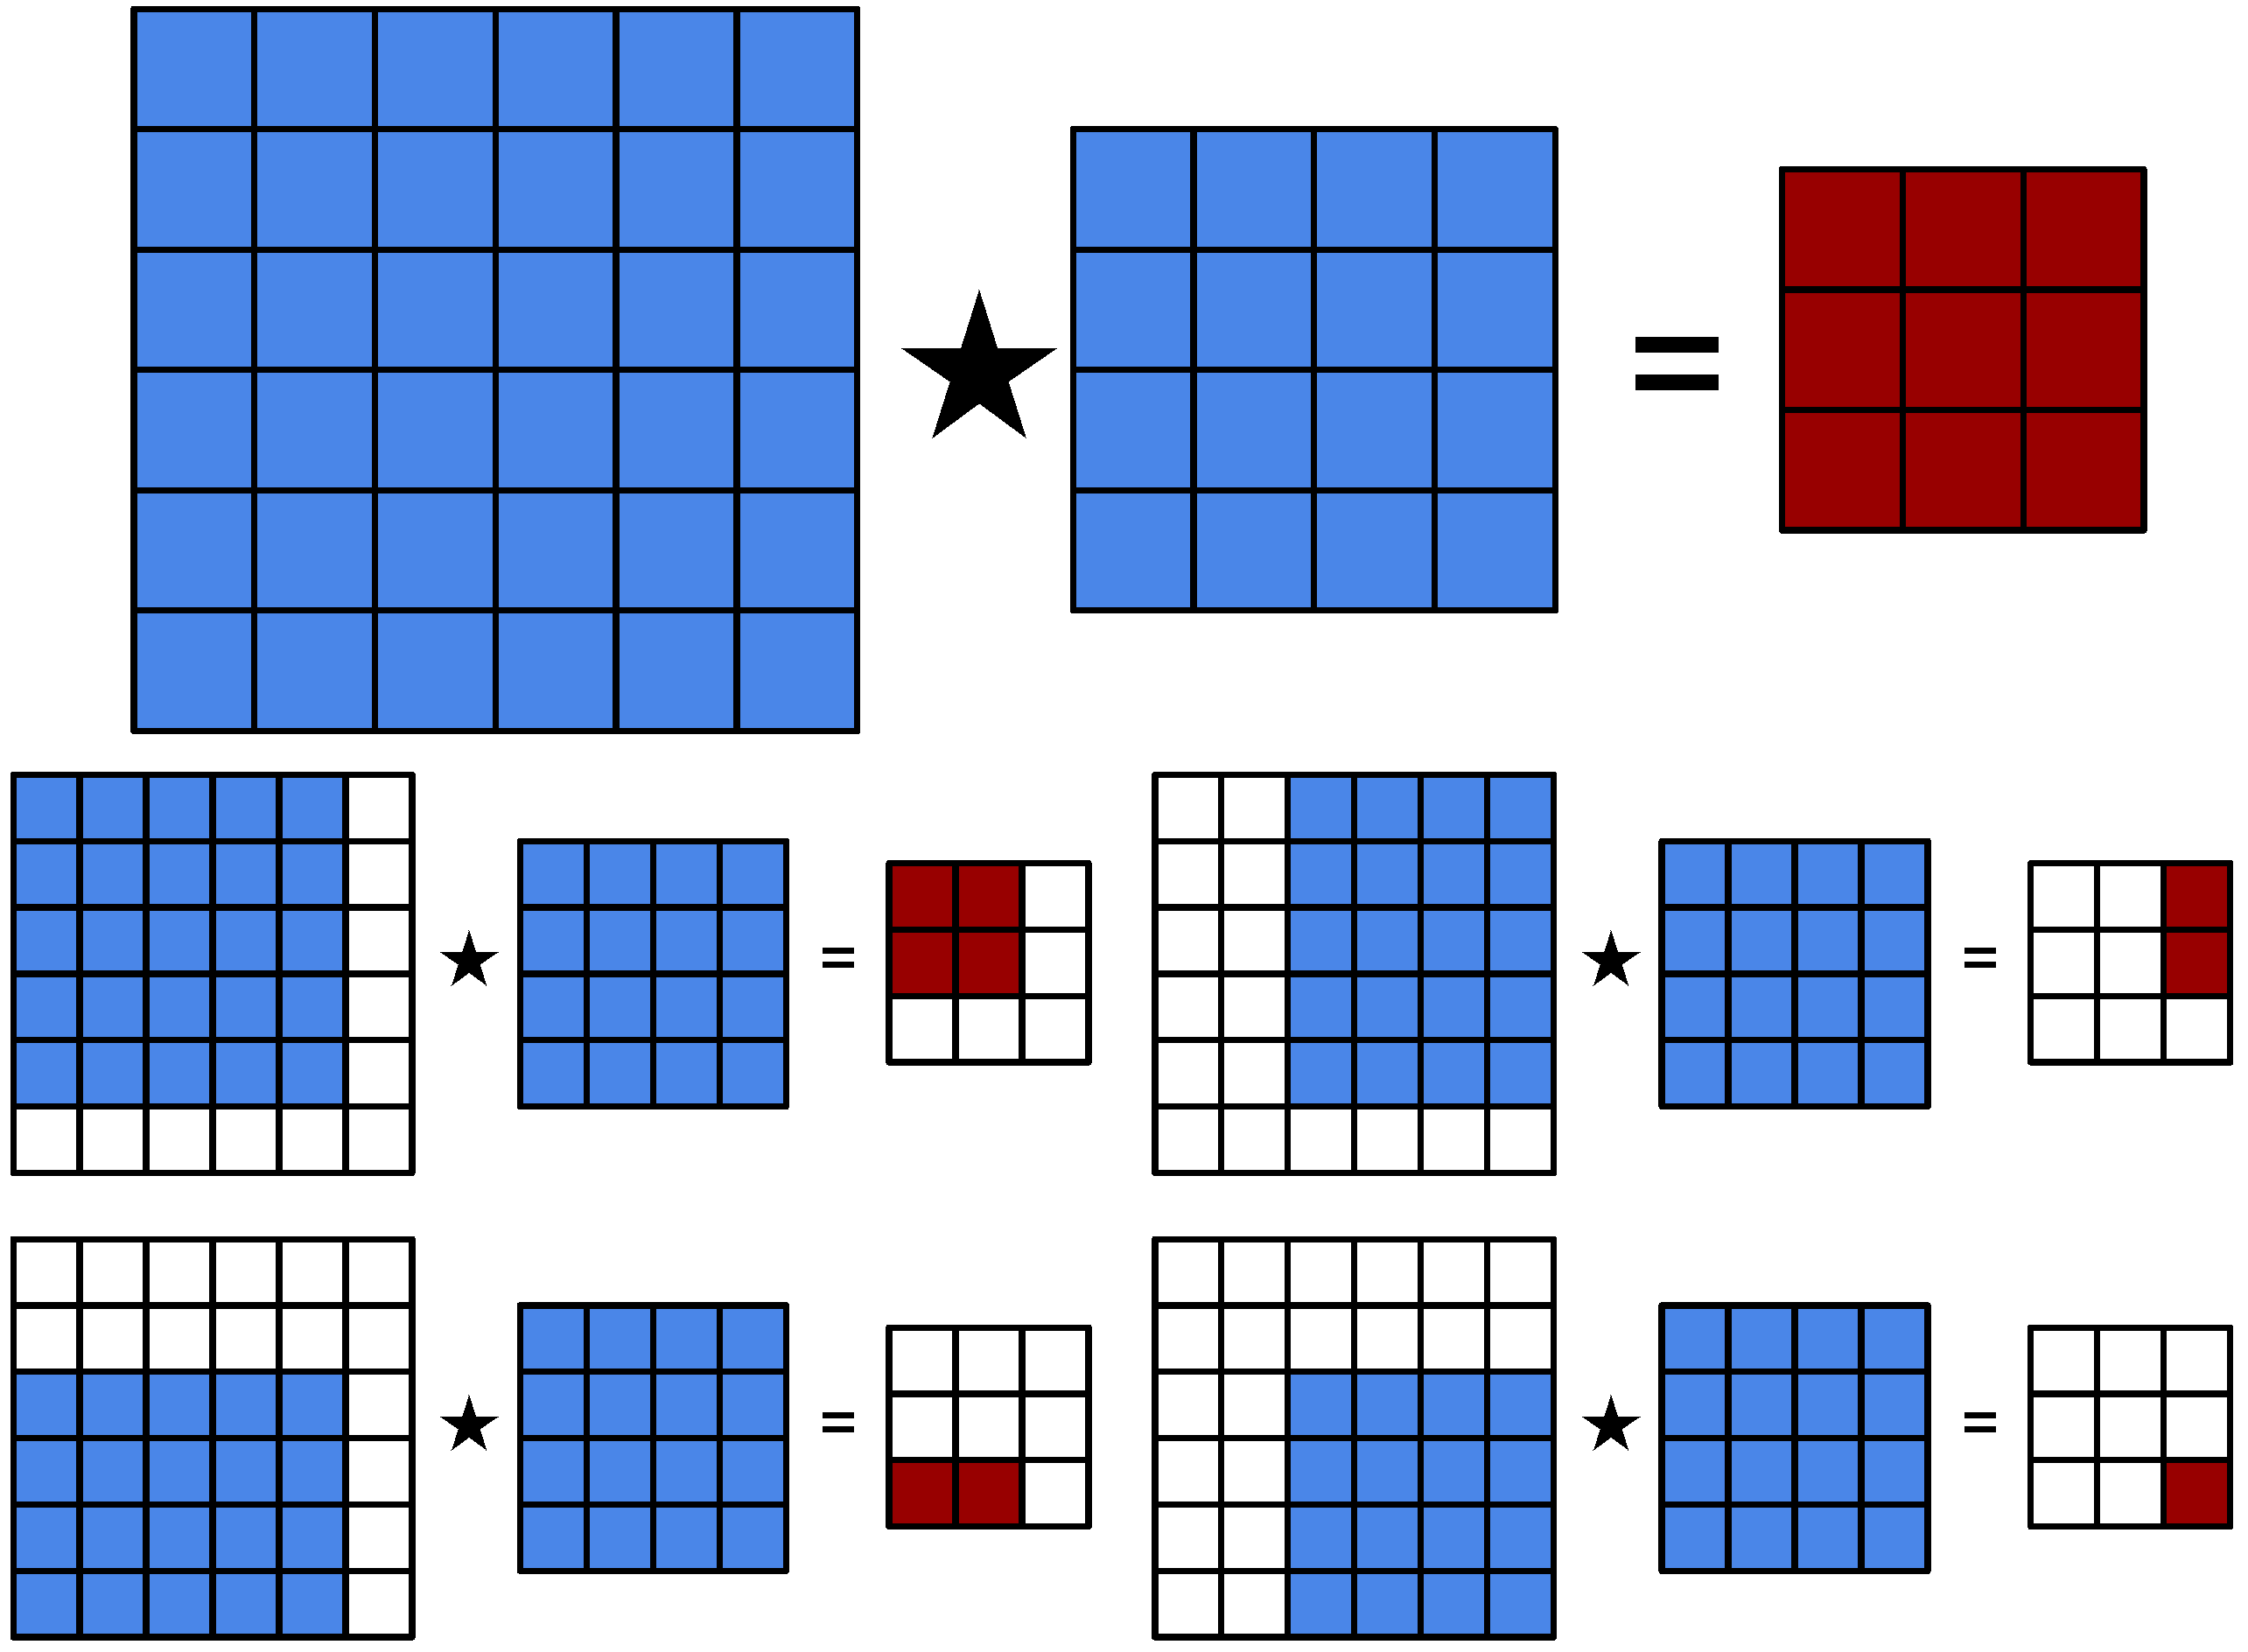
\includegraphics[width=0.57\linewidth]{fig/division}
    \end{center}
    \caption{Computing sub--results of cross--correlation as
      cross--correlation of sub--images.}
    \label{fig:conv-division}
  \end{figure}

  {\bf Full image primitive} performs $S^2$ cross--correlations on $S$ images
  of an arbitrary size, producing $S$ output images of size $N_x'
  \times N_y' \times N_z'$.  This is done by dividing the output
  images into small sub--images (Fig~\ref{fig:conv-division} and using
  the primitive described above.  The size of each sub--image should
  be maximized, but is subject to constraints described above.  We
  prefer division into sub--images with large values of the least
  significant dimension, such that the adjacent pixels are adjacent in
  memory, thus benefit from hardware pre--fetching.  As the image
  dimensions are typically larger than $R$ (number of registers
  available for $oreg$, as described above), in most case, the image
  will be split into sub--images of size $1 \times 1 \times R$.
  Alternatively, we will try the subdivision into $1 \times 2 \times
  \floor{R/2}$, etc...  Note that in most cases we will not be able to
  subdivide the image into equal parts.  This is handled by
  instantiating separate primitives for different sub--image sizes.
  This will result in the image fully covered in tiles, not all of
  which will have the same size.  However, we will have an optimally
  compiled code for each of them.

  The computation is then performed tile by tile, sliding along the
  least significant direction first, then the second least
  significant, etc...  This order of computation has multiple
  benefits.  First, it can benefit from hardware pre--fetching.
  Secondly, accessing contiguous data minimizes possible cache
  associativity conflicts, allowing us to store more data in the
  higher levels of cache.  This values can be reused as we slide along
  the more significant dimensions.

  {\bf Sub--layer primitive} considers all $\alpha S$ input images and
  computes the values of $\beta S$ ($\beta \le \alpha'$) output
  sub-images of size $N_x' \times N_y' \times N_z'$ by performing
  $\alpha \beta S^2$ cross--correlations.  This is achieved by invoking
  $\alpha \beta$ {\bf full image primitives} described above.

  \begin{figure}
    \begin{center}
      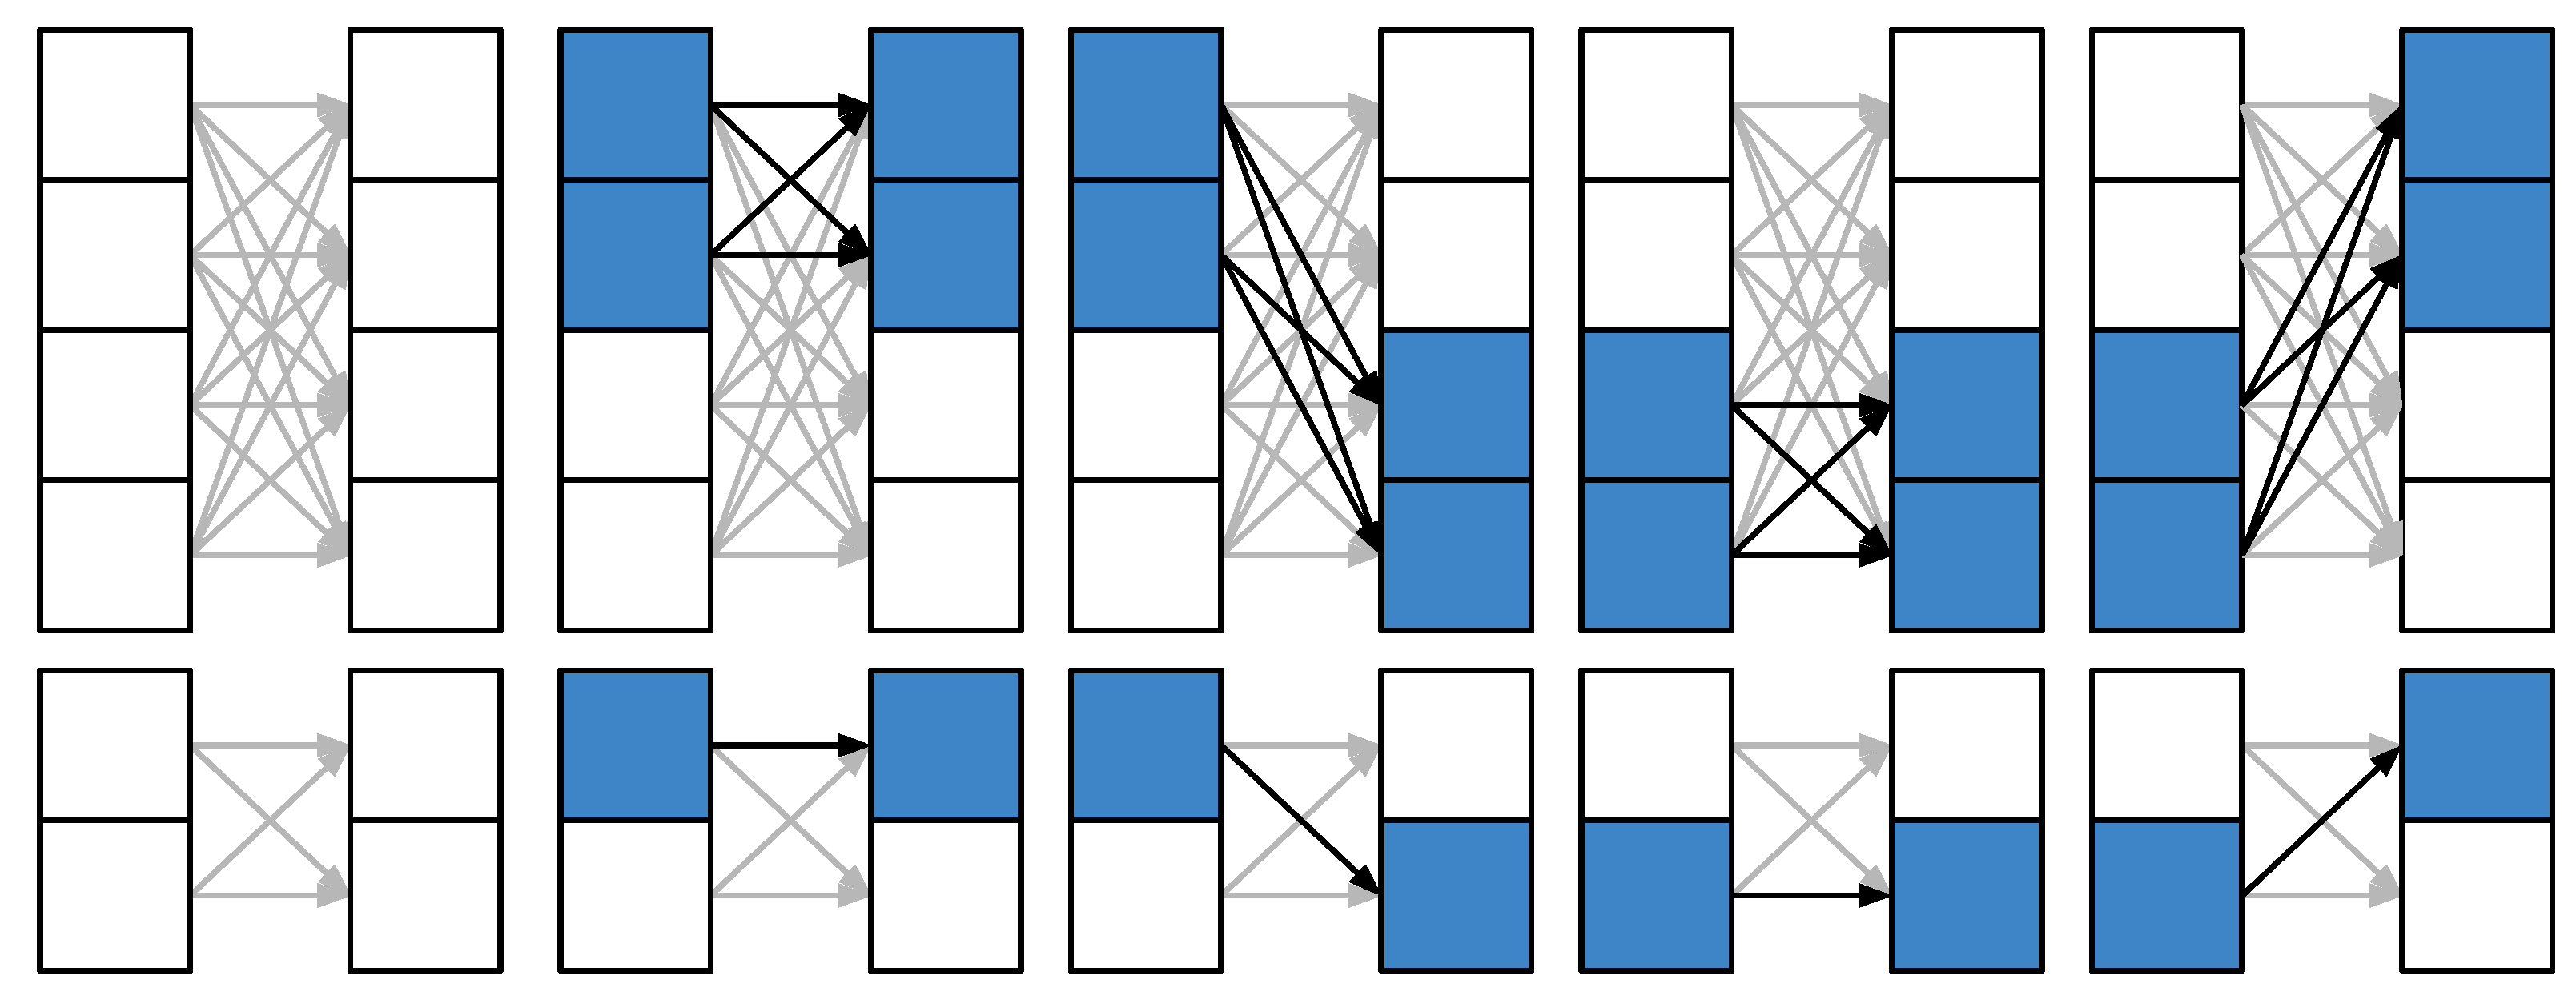
\includegraphics[width=0.8\linewidth]{fig/serialexec}
    \end{center}
    \caption{The recursive computation done by sub--layer primitive.
      Two levels of recursion are shown, each requiring less cache. }
    \label{fig:full-exec}
  \end{figure}

  This primitive is designed to efficiently use higher levels of cache
  when available, by ensuring that the order of {\bf full image
    primitives} are executed in a cache--friendly way.  This is
  achieved in a recursive fashion, where each successive recursive
  step requires half the memory to fit the whole working set inside
  the cache.  Two levels of recursion are shown for the case of
  $\alpha = \beta = 4$ are shown on Fig.~\ref{fig:full-exec}.  In the
  first step (first row in Fig.~\ref{fig:full-exec}), both the number
  of input and output images are divided in half.  The next recursive
  step (second row in Fig.~\ref{fig:full-exec}) is then applied for
  all 4 possible subdivisions.  Note how the second level of recursion
  requires storage for 2 input and 2 output images in order to fit the
  whole working set inside cache, while the first level requires twice
  as much.  The order in which the 4 recursive problems are solved
  further increases cache reuse.  In the case when $\alpha \ge 2\beta$
  or $\beta \ge 2\alpha$ a simpler recursive step is performed, by
  dividing only the input/output images in half and solving two
  recursive sub--problems.

  {\bf Full layer primitive} divides the computation of $B$ sets of
  $\alpha' S$ output images into sets of sub--layer primitives.  Each
  of $T$ available threads is given an ordered list of primitives to
  execute.

  The main goal of the primitive is to equally divide the work among
  the $T$ threads such that once invoked they all finish roughly at
  the same time.  As described above, the $B$ sets of $\alpha'S$
  output images of size $N_x' \times N_y' \times N_z'$ can regarded as
  a $5D$ tensor of size $B \times (\alpha'S) \times N_x \times N_y
  \times N_z$.  We take a recursive approach to our static scheduling
  algorithm.  The input to our algorithm is a set of $T$ threads, and
  a $5D$ tensor of values that has to be computed.

  For the base case of our algorithm, when $T=1$, a sub--layer
  primitive that computes the values of the $5D$ tensor is {\bf
    appended} to the list of primitives to be executed by the given
  thread.

  Our algorithm has two different recursive steps.  The first version
  of the recursive step first finds the smallest prime $p$ that
  divides $T$.  It then divides the set of $T$ threads into $p$ sets
  of $T/p$ threads, and the $5D$ tensor into $p$ equal sub--tensors by
  slicing it along the highest significant dimension that has a size
  of at least $p$.  It then recursively solves the $p$ sub--problems
  for each set of $T/p$ threads and each equally sized sub--tensor.
  If no dimension of the tensor is larger or equal than $p$, we apply
  the base case on an arbitrary available thread.  If the dimension of
  the tensor along which the splicing was performed is not divisible
  by $p$, another recursive problem is solved for all $T$ threads and
  the remaining sub--tensor.  Note that the size of the sub--tensor of
  each recursive sub--problem has at least $p$ times less elements.

  The assigned lists of primitives to be executed by each thread will
  be exponentially smaller in size, with possibly some threads
  executing an extra, computationally cheap primitives.  Thus, we
  expect the threads to be done roughly at the same time.

  As our previous primitives assume computation of multiple of $S$
  images, splicing along the second most significant dimension (of
  size $\alpha'S$) is done only when $\alpha' \ge p$.

  Note that in the last recursive call for the remainder of the
  sub--divided tensor, the value of $T$ doesn't decrease.  The depth
  of recursion can reach up to $\log_2 E$, where $E$ is the number of
  elements in the $5D$ tensor, which can be very large.  As the
  scheduling is done during compile--time, this can significantly
  increase the compile time, and create ``code bloat''.

  To prevent this we introduce the second version of the recursive
  step, which is applied when the number of elements of the $5D$
  tensor is very small (compared to the original tensor).  In this
  case we divide the tensor along the most significant dimension
  larger than $T$ into $T$ sub--tensors, some of which are larger than
  others, after which $T$ base cases are applied and the work is
  scheduled on the $T$ threads.  The basic idea is that once
  computation required for the sub--tensor is small compared
  ($\epsilon$ times smaller) to the overall computation required for
  the whole layer, we can allow for some cores to do a bit more work
  than others without hurting overall performances.  In our
  implementation we chose $\epsilon = 0.008$.  This limits the
  recursion to maximal depth of $7$ while not allowing any single core
  to perform more then $1\%$ more work than other cores.

  \begin{figure}
    \begin{center}
      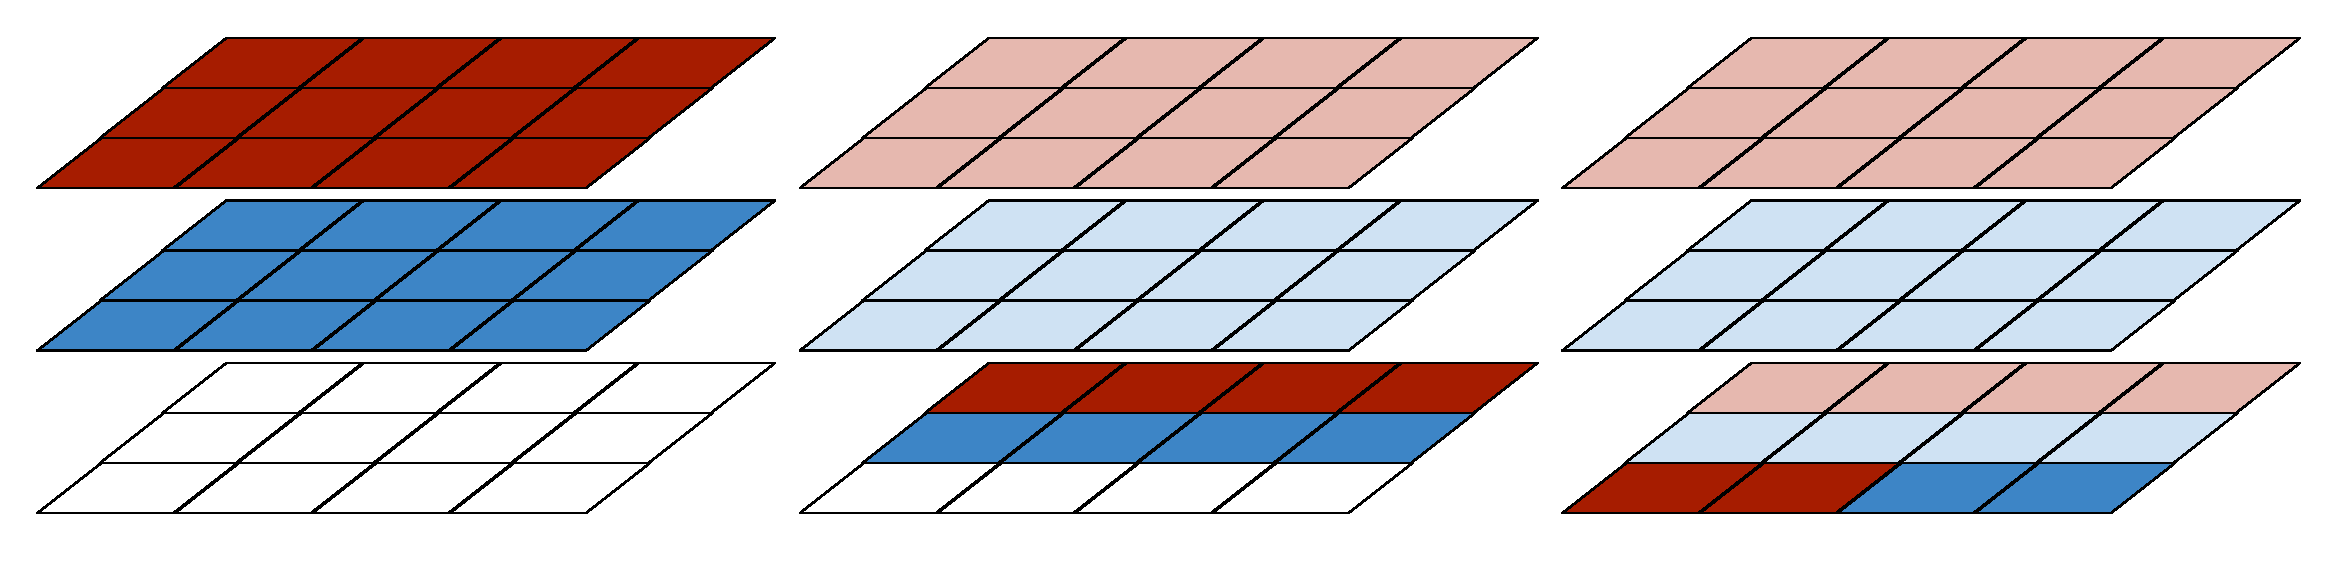
\includegraphics[width=0.67\linewidth]{fig/static2}
    \end{center}
    \caption{Computing the values of $F'=3$ channels of 2D images of
      size $4 \times 3$ using $T=2$ threads.  The three columns
      represent three stages.  The dark blue/red represent the values
      scheduled to be computed by $1^{st}/2^{nd}$ core.}
    \label{fig:problem-subdivision}
  \end{figure}

  An example of such scheduling for the special case of $B=1$, $F'=3$
  and $S=1$ and 2D images of size $4 \times 3$ is shown on
  Fig.~\ref{fig:problem-subdivision}.

  There are multiple benefits of our approach.  First, note that all
  the cores perform exactly the same computation.  When using multiple
  virtual threads per physical core, each thread can benefit from $L1$
  instruction cache.  Additionally, when multiple threads compute
  different images of the layer (as in the first step in
  Fig.~\ref{fig:problem-subdivision}), they access the elements of the
  input images in the exact same order.  This will yield high hit rate
  of the higher levels of cache shared between cores.

  \subsection{Input image padding and strided convolution}

  As mentioned before, in order to be usable for the backward pass,
  our primitive has to support either implicit or explicit zero
  padding of input images.  When the input images are large, and
  kernels small, explicit zero padding of the input image only
  slightly increases the computational cost.  However, as the images
  get smaller this overhead can become significant.

  We support implicit padding along an arbitrary of dimensions by
  modifying the lines 8--11 of
  Algorithm~\ref{alg:serial-forward-subtask}.  Instead of looping over
  all possible kernel offsets, for each invocation of the primitive,
  we provide additional run--time parameters, a pre--computed limits,
  for which the kernels offset are valid.

  Additionally, once might consider a hybrid approach, where along
  some directions the input is explicitly padded, while along the
  other we perform implicit computation.

  Our algorithm can easily be modified to support strided
  convolution/cross--correlation, which is supported in our
  implementation.  This is accomplished by simply modifying the line
  $18$ of Algorithm~\ref{alg:serial-forward-subtask} to account for
  the strides.

\section{Update phase}

  While the forward and backward pass perform cross--correlations and
  convolutions with a relatively large image with a small kernel
  producing another relatively large image, the cross--correlations
  performed during the update phase are performed on a large image
  with another large image resulting in a small image.

  Similarly as in the propagation algorithm, our update phase algorithm
  consists of the following stack of primitives.

  \begin{enumerate}
    \item {\bf Sub--kernel primitive} -- a primitive that computes a
      cross--correlation of each of $S$ images of size $R_Z \times R_Y
      \times (X + R_X - 1)$ with $S$ gradients of size $1 \times 1
      \times X$ to produce and accumulate the results of $S^2$ kernel
      gradients of size $R_Z \times R_X \times R_Y$.  As in the
      propagation algorithm, this primitive is optimized for efficiently
      reusing the register file as well as $L1$ cache.
    \item {\bf Full kernel primitive} -- a primitive that computes
      cross--correlation of an arbitrary sized $S$ images with
      arbitrary sized $S$ gradients to produce $S^2$ kernel gradients.
    \item {\bf Sub--layer primitive} -- a primitive that computes
      $\alpha \times \beta \times S^2$ kernel gradients by
      cross--correlating each of $\alpha S$ images with $\beta S$
      gradients.
    \item {\bf Full layer primitive} -- parallelized primitive that
      divides the computation into a set of previous primitives and
      statically schedules execution.  As described below, this
      primitive might need to contain an extra parallelized reduction
      step, which is also statically scheduled.
  \end{enumerate}


  \begin{algorithm}
    {\footnotesize
      \begin{codebox}
        \Procname{$\proc{Update-Subtask} \langle R_x, R_y, R_z, Z, R_s \rangle(i,og,wg^T)$}
        \li \kw{simd register} $oreg[R_x][R_y][R_z][R_s]$
        \li \kw{simd register} $wreg$
        \li \For $s_0 \gets 0 \To S/R_s - 1$
        \li \Do $oreg[:][:][:][s_0R_s:s_0R_s+R_s-1][:] \gets$
        \li   \Do $\proc{LOAD}(wg^T[:][:][:][s_0R_s:s_0R_s+R_s-1][:])$
        \End
        \li \For $z_g \gets 0 \To Z-1$ \Comment Partially unrolled
        \li   \Do $wreg \gets \proc{LOAD}(og[1][1][z_g][:])$
        \li   \For $x \gets 0 \To R_x-1$ \Comment Fully unrolled
        \li   \Do \For $y \gets 0 \To R_y-1$  \Comment Fully unrolled
        \li   \Do \For $z \gets 0 \To R_z-1$  \Comment Fully unrolled
        \li   \Do \For $s_1 \gets 0 \To R_S-1$   \Comment Fully unrolled
        \li   \Do $oreg[x][y][z][s_0 \cdot R_s + s] \gets \proc{FMADD}($
        \li   \Do $wreg,$
        \li       $\proc{EXLOAD}(i[x][y][z+i][s_0 \cdot R_s + s]),$
        \li       $oreg[x][y][z][])$
        \End
        \End \li \kw{end for} $s$
        \End \li \kw{end for} $x$
        \End \li \kw{end for} $y$
        \End \li \kw{end for} $z$
        \End \li \kw{end for} $i$
        \li $wg^T[:][:][:][s_0R_s:s_0R_s+R_s-1][:] \gets$
        \li \Do $\proc{STORE}(oreg[:][:][:][s_0R_s:s_0R_s+R_s-1][:])$
        \End
        \End \li \kw{end for} $s_0$
      \end{codebox}
    \caption{Serial update subtask.}
    \label{alg:serial-update-subtask}
    }
  \end{algorithm}

  {\bf Sub--kernel primitive} \quad The lowest level primitive is
  shown in Algorithm~\ref{alg:serial-update-subtask}.  Following the
  same principles as in the propagation sub--kernel primitive we
  vectorize the computation of $wg^T[r_x][r_y][r_z][f][f']$ computed
  via {\small
  \[
  \sum_{z}
  a[r_x][r_y][r_z+z][f] \cdot b[r_x][r_y][r_z][f']
  \]
  } such that the values of $wg^T[r_x][r_y][r_z][f][:]$ are computed
  via {\small
  \[
  \sum_{z}
  a[r_x][r_y][r_z+z][f] \cdot b[r_x][r_y][r_z][:]
  \]
  } Again, we recognize the reuse of $og[r_x][r_y][r_z][:]$ and
  re--order the loops appropriately.  In order to allow in--register
  computation, same constraints are imposed on $R_x \times R_y \times
  R_z \times R_s$ -- Maximal of $31$ for AVX512 and $8$ for SSE4, AVX
  and AVX2.  Additionally we allow only values for $R_s$ that divide
  $S$.  In order for the working set to fit inside the $L1$ cache, $Z$
  should be sufficiently small.  The number of bytes required for the
  working set equals $4S(R_xR_y+1)(R_z+Z-1)$.  For a given choice of
  $R_x, R_y$ and $R_z$, and given size of $L1$ cache, we
  conservatively choose $Z$ so that no more than half the cache is
  required for the working set.

   \begin{figure}
     \centering
     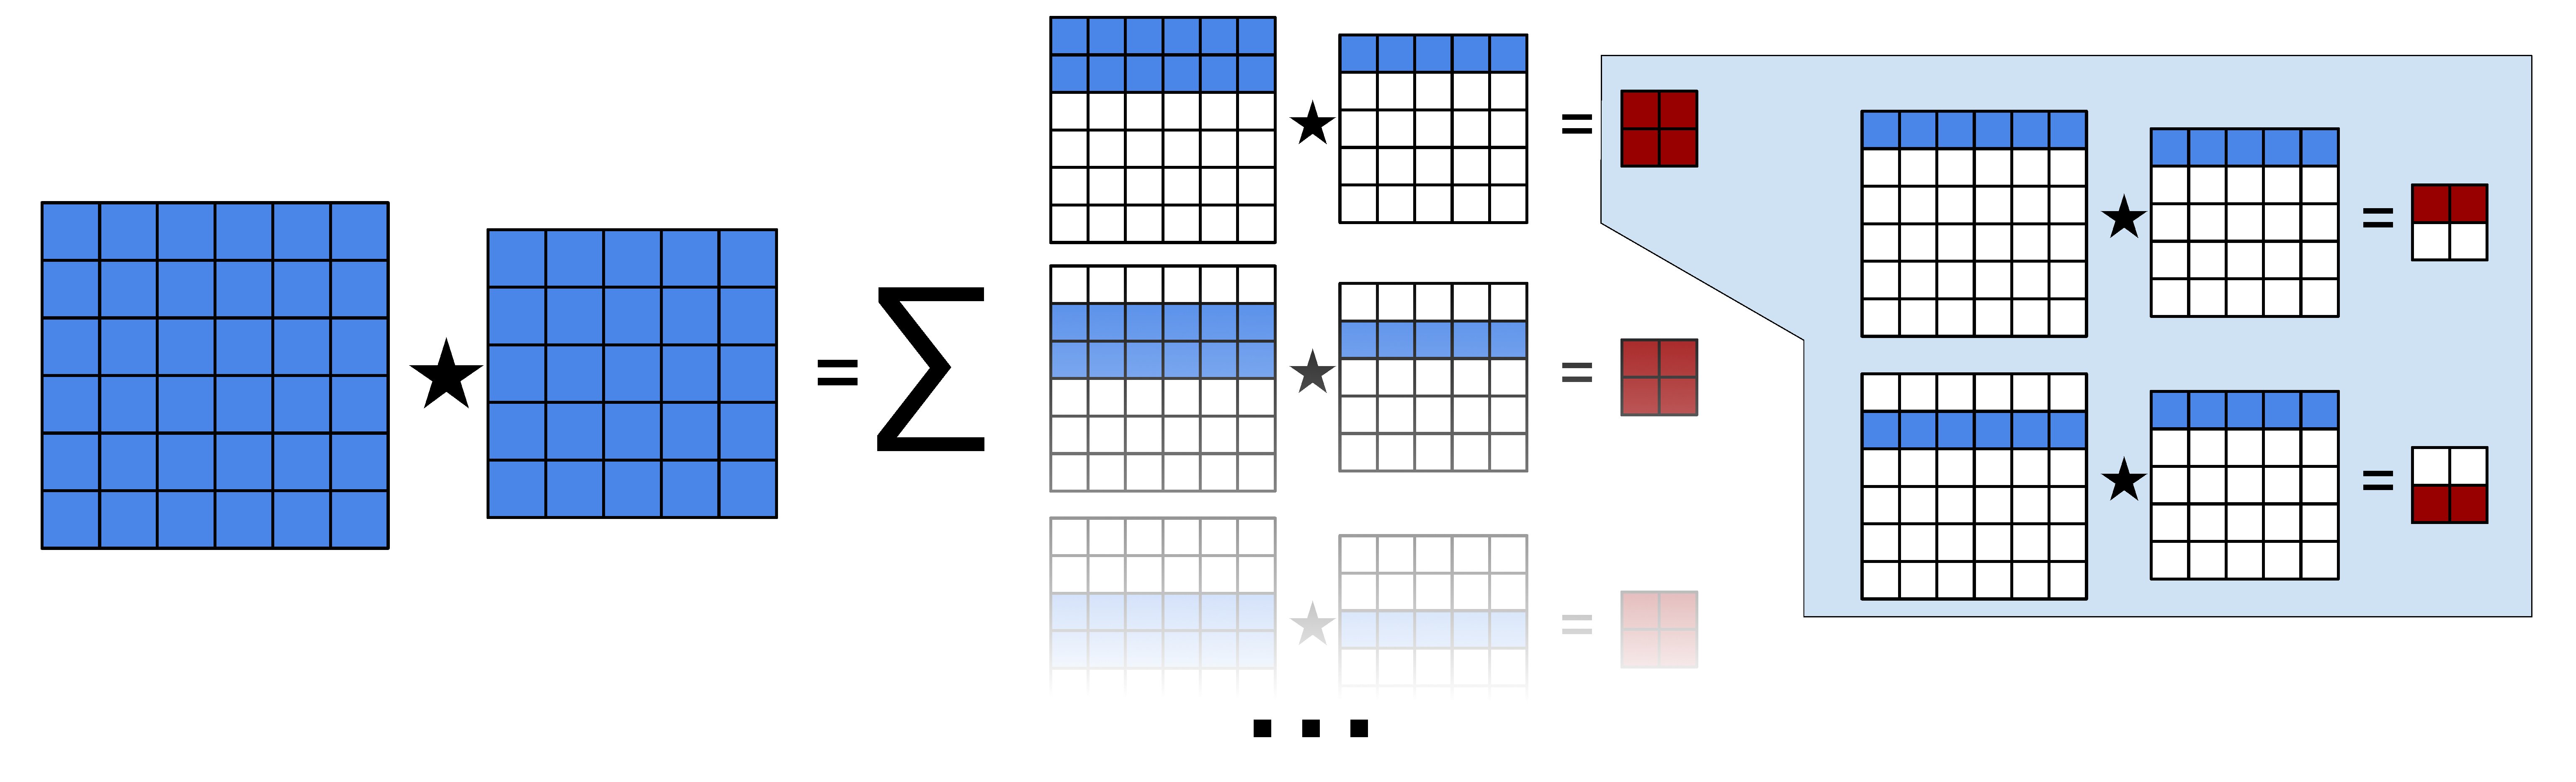
\includegraphics[width=0.99\linewidth]{fig/update2}
     \caption{An example of the {\bf full kernel primitive} and {\bf
         full gradient primitive} for the special case of $S=1$,...}
     \label{fig:conv-decomposition}
   \end{figure}

  {\bf Full kernel primitive} computes $S^2$ kernel gradients by
  cross--correlating each of $S$ images with $S$ gradients.  The
  computation is performed in two steps.  First, the gradients are
  split into sub--gradients of size $1 \times 1 \times Z$.  The result
  is then obtained as the sum of cross--correlations of each of the
  sub--gradients with an appropriate sub--image, as depicted on
  Fig~\ref{conv-decomposition} (middle column).  The
  cross--correlation of each sub--gradient is further split into
  sub--kernel primitives (right column on
  Fig.~\ref{conv-decomposition}.  We choose the $R_x, R_y, R_z$ and
  $R_s$ to maximize the register--file utilization, but subject to the
  limits described above.  Further, we require that $R_x, R_y$ and
  $R_z$ divide $K_x, K_y$ and $K_z$ respectively.  Note that this can
  always be accomplished be setting $R_x=R_y=R_z=1$ and $R_s=S$.
  However this choice might not be optimal.  For example, when $K_z=3$
  on AVX512 CPU, we could pick $R_s=8$ and $R_z=3$, which utilizes
  $24$ registers, which is better than choosing $R_z=1$ and
  $R_s=S=16$.  The optimal division is the one for which $R_x \times
  R_y \times R_z \times R_s$ is maximized.  When more combinations are
  possible, we prefer ones with large values of $R_s$, then $R_z$
  etc...  The value for $Z$ is then obtained using as described above.

  The computation is performed by iterating over the least significant
  dimension, then second least significant, etc..

  {\bf Sub--layer primitive} performs $\beta S \beta' S$
  cross--correlation.  Each of $\beta S$ input images is
  cross--correlated with each of $\beta'S$ output gradients to produce
  $\beta S \beta' S$ kernel gradients.  This primitive is designed for
  maximal reuse of higher levels of cache.  To achieve that, the
  computation is performed in the same fashion as in the propagation
  sub--layer primitive (Fig.~\ref{fig:full-exec}).

  {\bf Full layer primitive}, as in the propagation algorithm, divides
  the computation into sub--layer primitives which are scheduled for
  execution on $T$ threads.  In the propagation algorithm, all the
  divisions were done by splitting the large output tensor, allowing
  each thread to perform an independent computation.  As our update
  sub--layer primitive always computes full kernel gradients, the only
  sub--division into independently computer results is possible along
  the two most significant dimensions of $\Delta W$ tensor.

  Further division can be accomplished by dividing the computation
  over the input images and output gradients.  A division can be
  performed across the batches $B$, such that each thread considers
  only a subset of batches.  The resulting kernel gradients are then
  computed by accumulating the result obtained by each thread.
  Similarly, a division can be performed across the input image/output
  gradient as in the case of the {\bf full kernel primitive}.  This
  division also requires accumulating the results.

  To optimally divide the computation among threads we propose a two
  step scheduling algorithm.  In the first step, division along the
  two most significant dimensions of $\Delta W$ is performed to obtain
  independent sub--problems.  Let $P = \proc{GCD}(T,\alpha\alpha')$,
  we first select $\beta$ and $\beta'$ such that they divide $\alpha$
  and $\alpha'$ respectively, and $\beta\beta'P = T$.  Out of all
  possible values we pick the one for which $|\beta -\beta'|$ is
  minimized.  The threads are then also divided into $P$ sets of
  $T'=T/P$ threads, each of which will compute $\beta\beta'S^2$ kernel
  gradients.

  The values of the kernel gradient tensor $\Delta W(A
  \beta'S:A\beta'S+\beta'S-S,B \beta S: B\beta S + \beta S -S, :,:,:)$ is
  performed by the $A + B \alpha / \beta$-th set of $T'$ threads.

  In the second step, we divide the computation of

  When $T'$ equals $1$



  In the case when $T' \neq 1$ a second division step is performed.  IT IS THE SAME!



  In the second step, we consider each of the $P$ sets of $T'$
  threads.  Kernel gradients to be computed by each subset is computed
  by cross--correlating each of $\beta S$ input images with $\beta'S$
  output gradients for each set of inputs in the batch of size $B$.

  Further sub--division can be accomplished by dividing the
  computation such that different threads process either different
  sets in the batch or to process sub--images as depicted in the
  middle column of Fig.~\ref{conv-decomposition}.  The final result is
  then obtained by accumulating the result obtained by each thread.
  This means that an additional ``reduction'' pass is necessary -- we
  need to accumulate $T'$ results obtained by each of the threads.  As
  we need to divide the problem into exactly $T'$ subproblems, the
  recursive scheduling approach used for the propagation is not
  possible.  Instead, to divide the problem as evenly as possible over
  the $T'$ threads we perform the following recursive approach, that
  is not guaranteed to divide the problem as evenly as in the fwd--bwd
  case.

\section{Experiments}

  For a variety of CPUs, we benchmarked the convolutional layers of
  several state-of-the-art ConvNets used for (1) 2D object detection,
  (2) 2D image segmentation, and (3) 3D spatiotemporal feature
  learning.

  \begin{table} \centering
    \setlength\tabcolsep{2.5pt}
    \begin{tabular}{cr !{\vrule width0.8pt} cccccc  }
      &  & B & F & F' & Image Size & Padding & Kernel Size  \\
      \hline
      \multirow{5}{*}{\rotatebox{90}{\textbf{VGG-a}}}
      & C2 & 64  & 64  &  128 & $\angled{112,112}$ & $\angled{1,1}$ & $\angled{3,3}$ \\
      & C3 & 64  & 128 &  256 & $\angled{56,56}$   & $\angled{1,1}$ & $\angled{3,3}$ \\
      & C4 & 64  & 256 &  256 & $\angled{56,56}$   & $\angled{1,1}$ & $\angled{3,3}$ \\
      & C5 & 64  & 256 &  512 & $\angled{28,28}$   & $\angled{1,1}$ & $\angled{3,3}$ \\
      & C6 & 64  & 512 &  512 & $\angled{28,28}$   & $\angled{1,1}$ & $\angled{3,3}$ \\
      \hline
      \multirow{5}{*}{\rotatebox{90}{\textbf{U-Net}}}
      & C1b & 1  & 64  &  64 & $\angled{570,570}$  & $\angled{0,0}$ & $\angled{3,3}$ \\
      & C2b & 1  & 128 &  128 & $\angled{282,282}$ & $\angled{0,0}$ & $\angled{3,3}$ \\
      & C3b & 1  & 256 &  256 & $\angled{138,138}$ & $\angled{0,0}$ & $\angled{3,3}$ \\
      & C4b & 1  & 512 &  512 & $\angled{66,66}$   & $\angled{0,0}$ & $\angled{3,3}$ \\
      & C5b & 1  & 1024 &  1024 & $\angled{30,30}$ & $\angled{0,0}$ & $\angled{3,3}$ \\
      \hline
      \multirow{5}{*}{\rotatebox{90}{\textbf{VGG-a}}}
      & C2a & 32  & 64  &  128 & $\angled{16,56,56}$ & $\angled{1,1,1}$ & $\angled{3,3,3}$ \\
      & C3a & 32  & 128 &  256 & $\angled{8,28,28}$ & $\angled{1,1,1}$ & $\angled{3,3,3}$ \\
      & C3b & 32  & 256 &  256 & $\angled{8,28,28}$ & $\angled{1,1,1}$ & $\angled{3,3,3}$ \\
      & C4a & 32  & 256 &  512 & $\angled{4,14,14}$ & $\angled{1,1,1}$ & $\angled{3,3,3}$ \\
      & C4b & 32  & 512 &  512 & $\angled{4,14,14}$ & $\angled{1,1,1}$ & $\angled{3,3,3}$ \\
      \hline
      \multirow{5}{*}{\rotatebox{90}{\textbf{Toy}}}
      & 2D1 & 64  & 48 &  96 & $\angled{114,114}$ & $\angled{0,0}$ & $\angled{3,3}$ \\
      & 2D2 & 64  & 48 &  96 & $\angled{58,58}$ & $\angled{0,0}$ & $\angled{5,5}$ \\
      & 2D3 & 64  & 48 &  96 & $\angled{58,58}$ & $\angled{0,0}$ & $\angled{11,11}$ \\
      & 3D1 & 32  & 48 &  96 & $\angled{10,30,30}$ & $\angled{0,0}$ & $\angled{2,3,3}$ \\
      & 3D2 & 32  & 48 &  96 & $\angled{10,20,20}$ & $\angled{0,0}$ & $\angled{3,5,5}$ \\
      \hline
    \end{tabular}
    \caption{Benchmarked convolutional layers.}
    \label{table:layers}
  \end{table}

  \begin{table}
    \begin{center}
      \setlength\tabcolsep{2.5pt}
      \begin{tabular}{lrrrr}
        \toprule
        CPU & Frequency & CPUs $\times$ Cores/Threads & GFLOPS\\
        \midrule
        i7-6700K (Skylake) & 4GHZ & 1 $\times$ 4/8 & 512\\
        $4\times$ E7-8890v3 (Haswell) & 2.5GHz & 4 $\times$ 18/36 & 5760\\
        Xeon Phi 7210 & 1.1GHz & 1 $\times$ 64/256 & 4505.6\\
        \toprule
        GPU & Frequency & CUDA cores & GFLOPS\\
        \midrule
        Titan X (Maxwell) & 1GHz & 3072 & 6600\\
        Titan X (Pascal) & 1.5GHz & 3584  &  11000\\
        \bottomrule
      \end{tabular}
    \end{center}
    \caption{CPUs and GPUs used for benchmarks.}
    \label{table:cpus}
  \end{table}

  The 2D object detection ConvNet was the VGG-A version of
  OxfordNet~\cite{simonyan2014very}, an
  ImageNet~\cite{imagenet_cvpr09,ILSVRC15} winner that is widely used
  for speed benchmarks~\cite{imagenetwinners}.  The 2D image
  segmentation ConvNet was U--Net~\cite{ronneberger2015u}, used for
  biomedical image segmentation.  The object detection network uses
  ``batch training'' (multiple sets of inputs at the time), and
  gradually downsampled images.  The segmentation network uses rather
  large images with $B=1$.  The 3D spatiotemporal feature learning
  network was C3D~\cite{maturana_iros_2015}.  For each network, we
  benchmarked the five most computationally expensive convolutional
  layers (Table~\ref{table:layers}).

  The above ConvNets use only kernel sizes of $3 \times 3$ or $3\times
  3\times 3$, and the number of images in a layer is always a power of
  two.  To make our benchmarks more general (see ``Toy'' of
  Table~\ref{table:layers}), we also include layers with kernel sizes
  $5 \times 5$ and $11 \times 11$, inspired by
  AlexNet~\cite{krizhevsky2012imagenet}, kernel size $2 \times 3
  \times 3$, inspired by VD2D3D~\cite{lee2015recursive}, and kernel
  size $3 \times 5 \times 5$.  We also include layers with number of
  images not equal to a power of two.

  In addition, we benchmark each layer on three generations
  of Intel Xeon processors (Table~\ref{table:cpus}).  All the machines
  except the Skylake CPU were set to run at constant frequency (we did
  not have root access to the Skylake machine). 

  \begin{figure*} \centering
    \small
    \setlength\tabcolsep{0.5pt}
    \begin{tabular}{ >{\centering\arraybackslash}c ccccccl }
      \toprule
      & \multicolumn{2}{c}{\textbf{Skylake}}
      & \multicolumn{2}{c}{\textbf{Haswell}}
      & \multicolumn{2}{c}{\textbf{Knights Landing}} & \\
      \midrule
      & Forward & Update & Forward & Update & Forward & Update & \\
      \midrule
      \rotatebox{90}{\qquad \textbf{VGG-A}}
      & 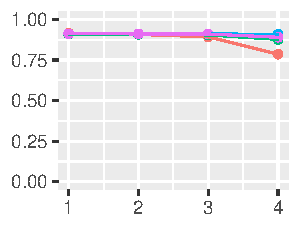
\includegraphics[height=2.4cm]{fig/vgg-fwd-skylake}
      & 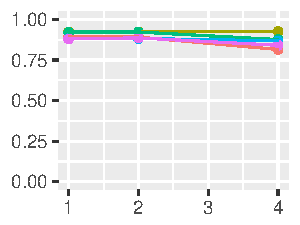
\includegraphics[trim=8mm 0mm 0mm 0mm,clip,height=2.4cm]{fig/vgg-upd-skylake}
      & 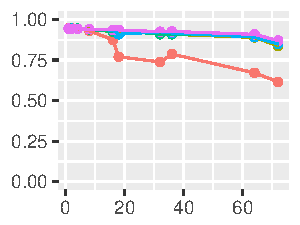
\includegraphics[trim=8mm 0mm 0mm 0mm,clip,height=2.4cm]{fig/vgg-fwd-haswell}
      & 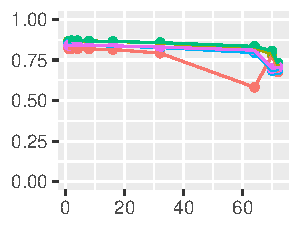
\includegraphics[trim=8mm 0mm 0mm 0mm,clip,height=2.4cm]{fig/vgg-upd-haswell}
      & 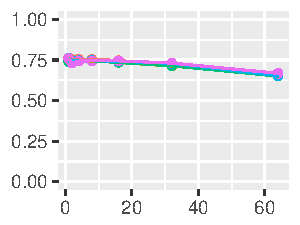
\includegraphics[trim=8mm 0mm 0mm 0mm,clip,height=2.4cm]{fig/vgg-fwd-knl}
      & 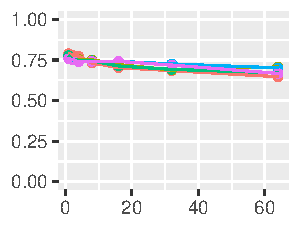
\includegraphics[trim=8mm 0mm 0mm 0mm,clip,height=2.4cm]{fig/vgg-upd-knl}
      & 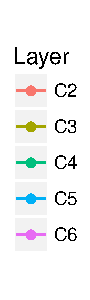
\includegraphics[height=2.4cm]{fig/vgg-legend} \\
      \midrule
      \rotatebox{90}{\qquad \textbf{U-Net}}
      & 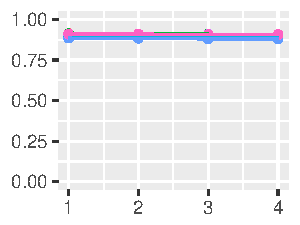
\includegraphics[height=2.4cm]{fig/unet-fwd-skylake}
      & 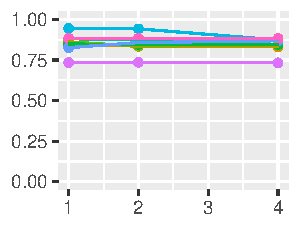
\includegraphics[trim=8mm 0mm 0mm 0mm,clip,height=2.4cm]{fig/unet-upd-skylake}
      & 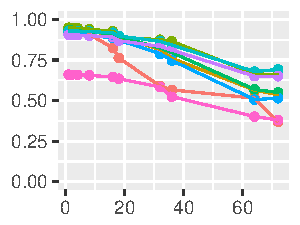
\includegraphics[trim=8mm 0mm 0mm 0mm,clip,height=2.4cm]{fig/unet-fwd-haswell}
      & 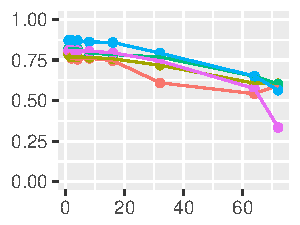
\includegraphics[trim=8mm 0mm 0mm 0mm,clip,height=2.4cm]{fig/unet-upd-haswell}
      & 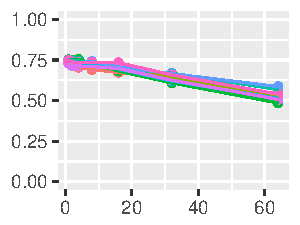
\includegraphics[trim=8mm 0mm 0mm 0mm,clip,height=2.4cm]{fig/unet-fwd-knl}
      & 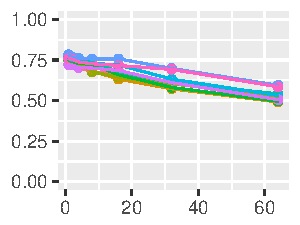
\includegraphics[trim=8mm 0mm 0mm 0mm,clip,height=2.4cm]{fig/unet-upd-knl}
      & 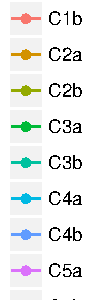
\includegraphics[height=2.4cm]{fig/unet-legend} \\
      \midrule
      \rotatebox{90}{\qquad \textbf{C3D}}
      & 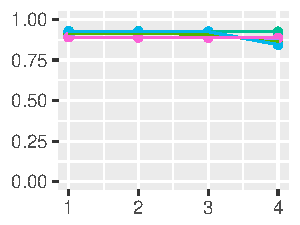
\includegraphics[height=2.4cm]{fig/d3d-fwd-skylake}
      & 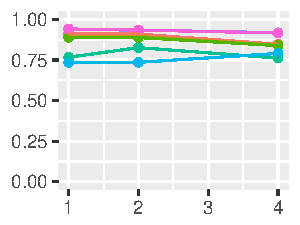
\includegraphics[trim=8mm 0mm 0mm 0mm,clip,height=2.4cm]{fig/d3d-upd-skylake}
      & 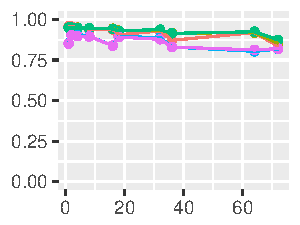
\includegraphics[trim=8mm 0mm 0mm 0mm,clip,height=2.4cm]{fig/d3d-fwd-haswell}
      & 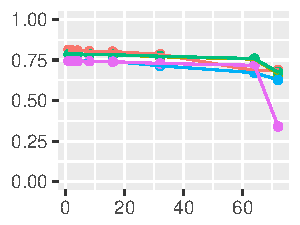
\includegraphics[trim=8mm 0mm 0mm 0mm,clip,height=2.4cm]{fig/d3d-upd-haswell}
      & 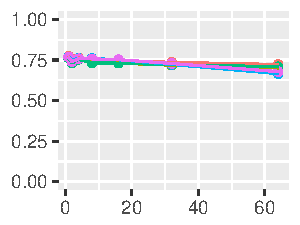
\includegraphics[trim=8mm 0mm 0mm 0mm,clip,height=2.4cm]{fig/d3d-fwd-knl}
      & 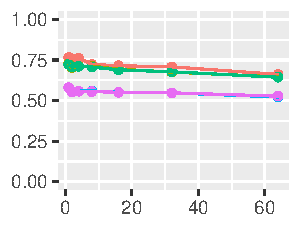
\includegraphics[trim=8mm 0mm 0mm 0mm,clip,height=2.4cm]{fig/d3d-upd-knl}
      & 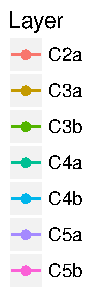
\includegraphics[height=2.4cm]{fig/d3d-legend} \\
      \midrule
      \rotatebox{90}{\qquad \textbf{Toy}}
      & 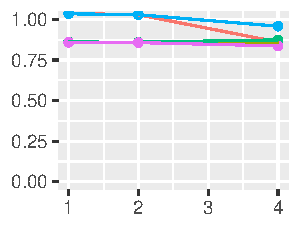
\includegraphics[height=2.4cm]{fig/toy-fwd-skylake}
      & 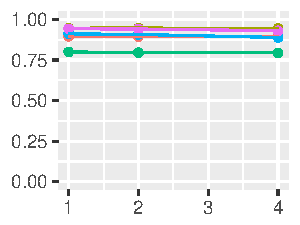
\includegraphics[trim=8mm 0mm 0mm 0mm,clip,height=2.4cm]{fig/toy-upd-skylake}
      & 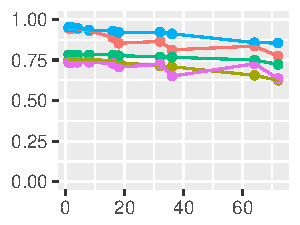
\includegraphics[trim=8mm 0mm 0mm 0mm,clip,height=2.4cm]{fig/toy-fwd-haswell}
      & 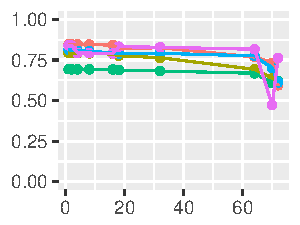
\includegraphics[trim=8mm 0mm 0mm 0mm,clip,height=2.4cm]{fig/toy-upd-haswell}
      & 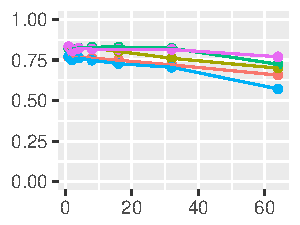
\includegraphics[trim=8mm 0mm 0mm 0mm,clip,height=2.4cm]{fig/toy-fwd-knl}
      & 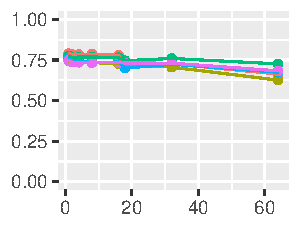
\includegraphics[trim=8mm 0mm 0mm 0mm,clip,height=2.4cm]{fig/toy-upd-knl}
      & 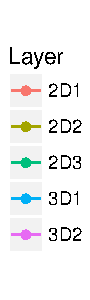
\includegraphics[height=2.4cm]{fig/toy-legend} \\
      \bottomrule

    \end{tabular}
    \caption{Utilization and scalability of our algorithms across
      different layers and CPU generations.  The $x$--axis represent
      number of cores used.  The $y$ axis represents the percentage of
      utilization of the used cores.}
    \label{fig:scalability}
  \end{figure*}

  \subsection{Benchmarking methodology}

  We benchmark both the propagation and the update algorithm for each
  layer on each CPU in the following way.  We compile the full layer
  primitive such that it uses only $N$ of the available cores and $H$
  hyper--threads per core.  We then perform 10 iterations of (1)
  randomly initializing all the data and (2) running the algorithm.
  We report the average time of running the second step.
  
  Randomly initializing the data before each iteration is important,
  as it clears the CPU caches.  Thus, our measurements represent a
  lower bound on the time required when the layer is part of a larger
  network that is being trained.  The speed of each primitive is
  computed by dividing the FLOPs required for the algorithm by
  average runtime.  The utilization is computed by dividing the speed
  of our algorithm (in FLOPS) by the FLOPS deliverable by $N$ cores of
  the given CPU.

  For Skylake and Haswell, we benchmarked our algorithm
  using gcc-5.3, icc-16 and clang-3.9.  The measured times were within
  a couple of percent, with icc-16 being the slowest, and clang-3.9
  being the fastest.  We report the gcc-5.3 numbers.

  For Xeon Phi, icc-16 and clang-3.9 performed equally well, with
  gcc-5.3 greatly under--performing.  Upon examining the generated
  assembly code, we noticed that gcc-5.3 failed to use the
  scalar--vector FMA instructions available.  The numbers reported are
  for icc-16.

  \subsection{CPU utilization and scalability}

  Utilization and scalability are shown in Fig~\ref{fig:scalability}.
  The $x$ axis represents the number of cores used, and the $y$ axis
  represents the percentage of utilization of the used cores.  A
  horizontal line would mean perfectly linear scalability.  For
  simplicity, points are only shown for the optimal number
  of hyper--threads per core, which was $2$ in more than 90\% of cases.
  More hyper--threads per core can hide memory latency, but will
  reduce effective cache sizes and might introduce cache associativity
  conflicts.
  
  In nearly all cases, single core utilization is higher
  than 75\%.  As we were unable to limit the CPU frequency on the
  Skylake CPU used for benchmarks, the turbo--boost that was enabled
  resulted in utilization higher than 100\% when one or two cores out
  of four available were used.

  Fig.~\ref{fig:scalability} suggest that our algorithms scale very
  well, with near linear scalability even for the multi--chip Haswell system.

  \subsection{Comparison versus other CPU implementations}

  We compare the speed of our approach to several competing CPU
  implementations for 2D ConvNets, CcT~\cite{hadjis2015shallow},
  MKL--DNN and MKL--2017.

% We are unable to compare the speed against
%  ZNN~\cite{zlateski2016znn} as it doesn't support layer--wise
%  computation, but rather parallelizes the whole training algorithm.
%  Also, we don't expect ZNN to be competitive as it is optimized for
%  large kernels.

  The CcT version of Caffe was used for benchmarking CcT.  The latest
  Intel--Caffe fork was compared separately for MKL-DNN and MKL-2017.
  Caffe benchmarks report the cumulative time of the backward
  propagation and update phase, so we report the numbers of our
  approach in the same fashion.  This is reasonable as in practice the
  backward pass and update phase are always performed one after the
  other.

  \begin{table} \centering
    \setlength\tabcolsep{2.5pt}
    \begin{tabular}{cr !{\vrule width0.8pt} rr|rr|rr|rr  }
      & & \multicolumn{2}{c|}{MKL-DNN} & \multicolumn{2}{c|}{MKL-2017}
      & \multicolumn{2}{c|}{CcT} & \multicolumn{2}{c}{Ours} \\
      &  & Fwd & B+U & Fwd & B+U& Fwd & B+U& Fwd & B+U \\
      \hline
      \multirow{5}{*}{\rotatebox{90}{\textbf{VGG-A}}}
      & C2  & 79.1  & 196.4 & 43.8 & 99.3  & 141.2 & 317.8 & {\bf 33.4} & {\bf 60.4}  \\
      & C3  & 42.4  & 106.8 & 30.0 & 78.5  & 118.5 & 194.3 & {\bf 24.5} & {\bf 60.3}  \\
      & C4  & 101.3 & 322.3 & 58.6 & 158.0 & 263.5 & 395.4 & {\bf 48.2} & {\bf 100.6} \\
      & C5  & 44.2  & 203.5 & 27.3 & 76.2  & 92.6  & 233.9 & {\bf 24.2} & {\bf 53.2}  \\
      & C6  & 89.8  & 466.5 & 54.8 & 149.9 & 196.8 & 466.3 & {\bf 47.2} & {\bf 104.2} \\
      \hline
      \multirow{5}{*}{\rotatebox{90}{\textbf{U-Net}}}
      & C1b  & 257.44 & 494.93 & 183.16 & 195.86 & 1739 &  542 & {\bf 9.02} & {\bf 18.12} \\
      & C2b  & 127.55 & 248.83 & 82.80  & 42.53  & 1052 & 1671 & {\bf 6.07} & {\bf 13.91} \\
      & C3b  & 66.17  & 126.35 & 38.48  & 25.20  & 2988 & 4645 & {\bf 5.47} & {\bf 13.41} \\
      & C4b  & 53.89  & 90.54  & 18.66  & 26.90  & 2172 & 4033 & {\bf 5.16} & {\bf 13.21} \\
      & C5b  & 19.34  & 77.86  & 9.24   & 22.09  & 1667 & 3198 & {\bf 4.35} & {\bf 11.23} \\
      \hline

    \end{tabular}
    \caption{Benchmarks of the 2D layers against CcT, MKL-DNN and
      MKL-2017 on the 4--way E7-8890v3 (Haswell) machine.}
    \label{table:2d-haswell}
  \end{table}

  On a 4--way Haswell machine, MKL--2017 was the best of the three
  competitors (Table~\ref{table:2d-haswell}), and our approach
  outperformed MKL--2017.  For VGG--A layers, MKL--2017 was not much
  slower (only 10-20\% for forward propagation, and 50\% for backward
  propagation + update).  For U-Net layers, our approach greatly
  outperformed MKL--2017, with up to $20\times$ greater speed
  for layer $C1b$ forward propagation.

  \begin{table} \centering
    \setlength\tabcolsep{2.5pt}
    \begin{tabular}{cr !{\vrule width0.8pt} rr|rr|rr  }
      & & \multicolumn{2}{c|}{MKL-DNN} & \multicolumn{2}{c|}{MKL-2017}
      & \multicolumn{2}{c}{Ours} \\
      &  & Fwd & B+U& Fwd & B+U& Fwd & B+U \\
      \hline
      \multirow{5}{*}{\rotatebox{90}{\textbf{VGG-A}}}
      & C2  & 101.9 & 266.8 & {\bf 34.6} & 101.8 & 40.1 & {\bf  80.7}  \\
      & C3  & 72.5  & 192.3 & {\bf 32.9} & 87.1  & 39.7 & {\bf  76.8}  \\
      & C4  & 142.0 & 402.9 & {\bf 65.4} & 166.2 & 80.6 & {\bf 158.9}  \\
      & C5  & 53.0  & 268.5 & {\bf 32.8} & {\bf 72.9}  & 40.1 & 77.5   \\
      & C6  & 108.3 & 557.3 & {\bf 64.8} & {\bf 172.3} & 78.6 & 157.3  \\
      \hline
      \multirow{5}{*}{\rotatebox{90}{\textbf{U-Net}}}
      & C1b  & 799.60 & 1603.93 & 141.01 & 61.96 & {\bf 9.89} & {\bf 21.81} \\
      & C2b  & 382.60 & 790.76  & 48.93  & 23.27 & {\bf 9.79} & {\bf 20.31} \\
      & C3b  & 187.08 & 421.61  & 23.10  & 16.84 & {\bf 8.50} & {\bf 16.71} \\
      & C4b  & 94.81  & 259.73  & 10.56  & 24.70 & {\bf 7.31} & {\bf 15.49} \\
      & C5b  & 44.01  & 167.88  & {\bf 5.45}   & {\bf 10.84} & 6.01 & 12.33 \\
      \hline

    \end{tabular}
    \caption{Benchmarks of the 2D layers against MKL-DNN and MKL-2017
      on the Xeon Phi 7210 machine.  CcT was not included as it did not compile for Xeon Phi.}
    \label{table:2d-knl}
  \end{table}

  For Xeon Phi, our approach was comparable to MKL-2017 for VGG-A
  layers, with MKL-2017 having a slight edge
  (Table~\ref{table:2d-knl}).  For U--Net layers, our approach was far
  superior to MKL-2017 on layers with fewer images, and was only
  slightly inferior on the widest layer with 1024 images.

  To summarize, our approach is far superior to competitors for
  training image segmentation architectures like U-Net.  For object
  detection architectures like VGG-A, our approach is slightly
  inferior to MKL-2017 for Xeon Phi KNL and slightly superior for
  4--way Haswell.

  \section{CPU vs. GPU for 3D convolutional layers}

  Finally, we compare the speed of 3D convolutional layers to state of
  the art 3D primitives for the GPU.  We used direct cuDNNv5 calls
  from C++, and the two latest generations of the Titan X GPU.

  \begin{table} \centering
    \setlength\tabcolsep{2.5pt}
    \begin{tabular}{cr !{\vrule width0.8pt} rr|rr !{\vrule width0.8pt} rr|rr  }
      & & \multicolumn{4}{c !{\vrule width0.8pt} }{\textbf{cuDNNv5 (Titan X)}} & \multicolumn{4}{c}{\textbf{Ours (Xeon)}} \\
      & & \multicolumn{2}{c|}{Maxwell} & \multicolumn{2}{c!{\vrule width0.8pt}}{Pascal}
      & \multicolumn{2}{c|}{Haswell} & \multicolumn{2}{c}{KNL} \\
      &  & Fwd & B+U & Fwd & B+U& Fwd & B+U& Fwd & B+U \\
      \hline
      \multirow{5}{*}{\rotatebox{90}{\textbf{C3D}}}
      & C2a & 186.8 & 370.3 & 168.0 & 336.0 & {\bf 147.6} & {\bf 325.2} & 218.1 & 456.3  \\
      & C3a & 90.1  & 180.0 & 78.5  & {\bf 161.2} & {\bf 72.2}  & 162.9 & 112.3 & 234.3  \\
      & C3b & 178.0 & 359.5 & 153.0 & 310.0 & {\bf 141.0} & {\bf 308.1} & 222.4 & 467.1  \\
      & C4a & 32.8  & 68.7  & 28.3  & {\bf 59.6}  & {\bf 27.7}  & 63.1  & 43.4  &  98.8  \\
      & C4b & 65.1  & 135.1 & 55.7  & {\bf 117.4} & {\bf 55.2}  & 131.2 & 85.3  & 196.1  \\
      \hline
    \end{tabular}
    \caption{3D vs GPU}
  \end{table}

\section{Conclusion and closing remarks}


\subsection{Implementation details}

\subsection{List of assumptions and design decisions}


%\clearpage
\bibliographystyle{./IEEEtran/IEEEtranBST/IEEEtran}
\bibliography{IEEEabrv,znnphi}
\end{document}
